\documentclass{article}

\usepackage{graphicx}
\usepackage{multimedia}
\usepackage{amssymb}

%\usepackage{algorithmic}
\usepackage{fancybox}
\usepackage{pseudocode}

\usepackage{pifont}
\usepackage{multirow}
\usepackage{slashbox}
\usepackage{pdfpages}
\usepackage{picture}

\title{CS566 Parallel Processing \\ Assignment 03}
\author{Camillo Lugaresi and Cosmin Stroe \vspace{20pt} \\ Department of Computer Science \\
University of Illinois at Chicago}

\date{November 8, 2011}

\begin{document}

\maketitle
\newpage

\section{Algorithm Details and Formulations}

For this assignment we tackled two main chanllenges.  The first was
experimenting with several implementations of matrix multiplication algorithms. 
In order to do matrix multiplication we implemented Cannon's algorithm and the
Dekel, Nassimi, Sahni (DNS) algorithm.  The second was the optimization of our
LU-decomposition algorithm by eliminating broadcast communication and using
pipelined communication instead.  The reason optimization of the
LU-decomposition algorithm became necessary was that we noticed that it was
taking significantly longer than the matrix multiplication algorithms.  As part
of our optimization we implemented a 1D row partitioning LU-decomposition
algorithm in addition to the 2D partitioning we had implemented for
Assignment 02.  We will be using timing results from both of these algorithms.

In our descriptions, we always refer to the formula $$C = A \times B$$ where
$A$, $B$, and $C$ are $n \times n$ matrices.  Some of the matrix multiplication
algorithms distribute the left and right matrices in a different manner and we
will make the distinction between $A$ and $B$, even though for our problem of
computing $A^k$ they contain identical values.  Our determinant is computed by
running the parallel formulation of the LU decomposition algorithm on the final
matrix, $A^k$.



\subsection{Cannon's Algorithm}

Cannon's algorithm is based on a checkerboard decomposition of the output data: the processors are arranged in a 2D mesh, and each is tasked with computing an $(n/\sqrt{p} \times n/\sqrt{p})$ block of the output matrix C.
To do so, each processor needs to access the corresponding row of blocks of matrix A and the corresponding column of blocks of matrix B:

$$C_{i,j} = \sum\limits_{k=1}^{\sqrt{p}} A_{i,k} \cdot B_{k,j}$$

A naive solution would be to have each processor store the entire row and column it needs, but that would be memory-inefficient. Instead, Cannon's algorithm distributes an $(n/\sqrt{p} \times n/\sqrt{p})$ block of A and one of B to the processor owning the block of C with the same coordinates, and relies on an intelligent schedule of communications and computations to ensure each processor gets the data it needs with no waste of memory and no dead times.

First, note that, by successively performing ring-1-shifts of the blocks of the A matrix on the row rings, and ring-1-shifts of the blocks of the  B matrix on the column rings, each processor gets to access all the blocks it needs. The problem is to ensure that the blocks are lined up so that the processor simultaneously holds the blocks of A and B that must be multiplied together.

As it turns out, this condition can be ensured for all processors at the same time by performing an initial skewing of the A and B matrices. Each row of A is shifted left by $i-1$ steps (where $i$ is the row number), and each column of B is shifted up by $j-1$ steps (where $j$ is the column number). At this point, each processor holds two blocks of A and B that must be multiplied together to form one term of the sum that produces $C_{i,j}$. Then all rows of A are shifted left by one step, and all columns of B are shifted up by one step; again, each processor ends up with a pair of elements that must be multiplied together and added to the computation of its $C_{i,j}$. These shift and multiply operations are repeated $\sqrt{p}$ times, until each processor has finished computing its block of C. Then the product matrix can be gathered.


\subsubsection{Local memory usage}

Each processor holds a block of the operand matrices A and B and of the result
matrix C. Therefore, $$M_p = O(n^2/p)$$

However, the root node is an exception
since it holds the initial matrix and gathers the final product matrix, so its
local memory usage is $$M_p = O(n^2)$$

\subsubsection{Parallel Computation Time (Local Computations)}

In the analysis of matrix multiplication it is usually assumed that the cost of
multiplication instructions dominates that of addition instructions; this
assumption is reflected in the reality of current computer systems.

For each invocation of the algorithm, each processor performs $\sqrt{p}$ naive
matrix multiplications of submatrices of size $n/\sqrt{p}$. Naive matrix
multiplication performs $O(n^3)$ multiplications, so the number of operations
per processor is $O(\sqrt{p}(n/\sqrt{p})^3)$. Then the computation time is: 

\begin{eqnarray*}
T_{{comp}} 	&=& t_{{mult}} \cdot \sqrt{p} \cdot (n/\sqrt{p})^3 \\ 
			&=& t_{{mult}} \cdot n^3 / p
\end{eqnarray*}

\subsubsection{Parallel Communication Time}

The algorithm involves the following communication steps:
\begin{itemize}
	\item scatter the X matrix into blocks of size $O(n^2/p)$
	\item skew matrix A (B); each processor performs a ring\_shift operation on
	the row (column) ring with distance = row (column) number
	\item $\sqrt{p}$ times: shift matrix A (B): ring\_shift with distance 1
	\item gather the product matrix
\end{itemize}

The message size $m$ is always $n^2/p$. In general, we can assume that $t_s$ is
dominated by $t_w \cdot m$.

\begin{itemize}
	\item Scatter on a mesh takes: $$T_{{scatter}} = t_s
\log{p} + t_w \cdot m  \cdot (p-1) = t_s \log{p} + t_w \cdot (n^2/p) \cdot
(p-1)$$
Gather has the same complexity as scatter.

\item Ring q-shift involves $\min(q, p-q)$ neighbor-to-neighbor communications:
$$T_{{shift-q}} = \min(q,p-q) \cdot (t_s + t_w \cdot m)$$

\item The highest value for the skew shift will be:
$$T_{{skew}} = \sqrt{p}/2 \cdot (t_s + t_w \cdot n^2/p)$$

\item For all of the $\sqrt{p}$ shifts collectively, we have
$$T_{{shift}} = \sqrt{p} \cdot (t_s + t_w \cdot n^2/p)$$

\end{itemize}

Then the overall communication time is:

\begin{eqnarray*}
T_{{comm}} 	&=& T_{{scatter}} + T_{{skew}} + T_{{shift}} + T_{{gather}} \\
			&=& 2 \cdot T_{{scatter}} + T_{{skew}} + T_{{shift}}  \\
			&=& 2 \cdot t_s  \cdot \log{p} + 2 \cdot t_w \cdot \frac{n^2}{p}(p-1) + \frac{\sqrt{p}}{2} \cdot (t_s + t_w \cdot n^2/p) + \sqrt{p} \cdot (t_s + t_w \cdot \frac{n^2}{p}) \\ 
			&=& 2 \cdot t_s \cdot \log{p} + 2 \cdot t_w  \cdot \frac{n^2}{p}(p-1) + \frac{3}{2}\sqrt{p}  \cdot \left(t_s + t_w \cdot \frac{n^2}{p}\right) \\ 
			&=& t_s \cdot \left(2 \log{p} + \frac{3}{2}\sqrt{p}\right) + t_w \cdot \left(2 \frac{n^2}{p}(p-1) + \frac{n^2}{p}\right) \\ 
			&=& t_s \cdot \left(2 \log{p} + \frac{3}{2}\sqrt{p}\right) + t_w \cdot \frac{n^2}{p}(2(p-1) + 1) \\
			&=& t_s \cdot \left(2 \log{p} + \frac{3}{2}\sqrt{p}\right) + t_w \cdot \frac{n^2}{p}(2p-1) \\
\end{eqnarray*}


\subsubsection{Parallel Run Time}

\begin{eqnarray*}
T_p 	&=& T_{{comp}} + T_{{comm}} \\
		&=& t_{{mult}} \cdot \frac{n^3}{p} + t_s \cdot \left(2 \log{p} + \frac{3}{2} \sqrt{p}\right) + t_w \cdot \frac{n^2}{p}(2p-1) \\
%		&=& O(n^3/p + \log{p} + \sqrt{p} + n^2 (2p-1)/p) \\
%		&=& O(n^3/p + \sqrt{p}) \\
\end{eqnarray*}

\subsubsection{Speedup}

For the reference serial algorithm, we will use the naive multiplication algorithm here.

\begin{eqnarray*}
S &=& \frac{T_s}{T_p} \\
&=& \frac{ t_{mult} \cdot n^3 }{ t_{mult} \cdot \frac{n^3}{p} + t_s \cdot \left(2 \log{p} + \frac{3}{2} \sqrt{p}\right) + t_w \cdot \frac{n^2}{p}(2p-1) } \\
&=& \frac{ n^3 }{ \frac{n^3}{p} + \frac{t_w}{t_{mult}} \cdot \frac{n^2}{p}(2p-1) + \frac{t_s}{t_{mult}} \cdot \left(2 \log{p} + \frac{3}{2} \sqrt{p}\right) } \\
&=& \frac{ p }{ 1 + \frac{t_w}{t_{mult}} \cdot \frac{2p-1}{n} + \frac{t_s}{t_{mult}} \cdot \frac{p\left(2 \log{p} + \frac{3}{2} \sqrt{p}\right)}{n^3} } \\
\end{eqnarray*}

%\begin{eqnarray*}
%S &=& T_s / T_p \\
%&=& \frac{n^3}{n^3 / p + \log{p} + \sqrt{p} + n^2 \cdot (2p-1)/p} \\
%&=& \frac{pn^3}{ n^3 + n^2 (2p-1) + p\sqrt{p} + p\log{p} } \\
%&=& \frac{p}{ 1 + \frac{2p-1}{n} + \frac{p(\sqrt{p} + \log{p})}{n^3} } \\
%\end{eqnarray*}

If $n$ grows much larger than $p$, the denominator approaches $1$, and so the system approaches linear speedup.

\subsubsection{Efficiency}

\begin{eqnarray*}
E &=& \frac{T_s}{pT_p} = \frac{S}{ p} = \\
&=& \frac{ 1 }{ 1 + \frac{t_w}{t_{mult}} \cdot \frac{2p-1}{n} + \frac{t_s}{t_{mult}} \cdot \frac{p\left(2 \log{p} + \frac{3}{2} \sqrt{p}\right)}{n^3} } \\
\end{eqnarray*}

If $n$ grows much larger than $p$, the system approaches ideal efficiency.

\subsubsection{Cost-optimality}

Cost-optimality is attained when efficiency remains constant as $n$ and $p$ change.
First, let us note that the impact of the startup time of communication is negligible when the message size is large; since our message size is $n^2/p$, this condition is satisfied. Therefore we can simplify the expression of efficiency as follows:

\begin{eqnarray*}
E &=& \frac{ 1 }{ 1 + \frac{t_w}{t_{mult}} \cdot \frac{2p-1}{n} } \\
\end{eqnarray*}

The condition for cost-optimality is then

\begin{eqnarray*}
O(2p-1) = O(n) \\
O(p) = O(n) \\
p = \Theta(n)
\end{eqnarray*}

Since our workload $W$ is $n^3$, the isoefficiency function can be obtained as

\begin{eqnarray*}
n &=& \Theta (p) \\
n^3 &=& \Theta (p^3) \\
W &=& k \cdot p^3 \\
\end{eqnarray*}


\subsection{Cannon's algorithm with local multiplication using Strassen}

\subsubsection{Local memory usage}

In addition to the normal memory usage for Cannon's algorithm, we must consider
the temporary storage used for Strassen. Strassen's algorithm is run locally by
each processor on a square block with size $n/\sqrt{p}$. Let us assume that
$n/\sqrt{p}$ is a power of 2.

Each invocation of Strassen on a matrix of size $s$ allocates storage for
$9 \cdot (s/2)^2$ elements (the 7 M matrices and two temporary matrices for computing
intermediate sums and products). Then it recursively invokes Strassen 7 times on
blocks of size $s/2$. Therefore its memory usage is:

\begin{eqnarray*}
f(s) &=& 9/4\cdot s^2 + 7\cdot f(s/2)	\\
&=& 9/4\cdot  s^2 + 7\cdot  9/4\cdot  (s/2)^2 + 7\cdot  7\cdot  f(s/4)	\\
&=& 9/4\cdot  (s^2 + 7/4\cdot  s^2) + 7\cdot  7\cdot  f(s/4)	\\
&=& 9/4\cdot  ( s^2 + 7/4\cdot  s^2 + (7/4)^2\cdot  s^2 ) +7^3\cdot  f(s/2^3) ... 	\\
&=& s^2 \cdot   9/4 \cdot   (7/4 + (7/4)^2 + \dots)	\\
&=& s^2 \cdot   9/4 \cdot   \sum\limits_{i=1}^{log_2 s} (7/4)^i 	\\
&=& s^2 \cdot   9/4 \cdot   log_2\left(2^{\sum\limits_{i=1}^{log_2 s} (7/4)^i}\right) 	\\
&=& s^2 \cdot   9/4 \cdot   log_2\left(\prod\limits_{i=1}^{log_2 s} 2^{(7/4)^i}\right) 	\\
&=& s^2 \cdot   9/4 \cdot   log_2\left(\prod\limits_{i=1}^{log_2 s} (7/4)^{2^i}\right) 	\\
&=& s^2 \cdot   9/4 \cdot   log_2(7/4) \cdot   log_{7/4}\left(\prod\limits_{i=1}^{log_2 s} (7/4)^{2^i}\right) 	\\
&=& s^2 \cdot   9/4 \cdot   log_2(7/4) \cdot   \left(\sum\limits_{i=1}^{log_2 s} log_{7/4}(7/4)^{2^i}\right) 	\\
&=& s^2 \cdot   9/4 \cdot   log_2(7/4) \cdot   \left(\sum\limits_{i=1}^{log_2 s} 2^i\right) 	\\
&=& s^2 \cdot   9/4 \cdot   log_2(7/4) \cdot   (2^{log_2 s+1} - 1) 	\\
&=& s^2 \cdot   9/4 \cdot   log_2(7/4) \cdot   (2 s - 1) 	\\
&=& s^2 \cdot   (2  s - 1) \cdot   9/4 \cdot   log_2(7/4) 	\\
&=& (2  s^3 - s^2) \cdot   9/4 \cdot   log_2(7/4)
\end{eqnarray*}

Hence
$$f(s) = O(s^3)$$

	
$$f(n/\sqrt{p}) = O\left(\frac{n^3}{p^{3/2}}\right)$$

Thus the space complexity becomes:
$$Mp = O\left(\frac{n^3}{p^{3/2}} + \frac{n^2}{p}\right) = O\left(\frac{n^2}{p} \cdot \left(\frac{n}{\sqrt{p}}+1\right)\right) = O\left(\frac{n^3}{p^{3/2}}\right)$$

For the root node, it becomes:

$$Mp = O\left(\frac{n^3}{p^{3/2}} + n^2\right) = O\left(n^2 \cdot \left(\frac{n}{p^{3/2}} + 1\right)\right) = O\left(\frac{n^3}{p^{3/2}}\right)$$


\subsubsection{Parallel computation time}

For each invocation of the algorithm, each processor performs $\sqrt{p}$ Strassen
matrix multiplications of submatrices of size $n/\sqrt{p}$. Strassen matrix
multiplication performs $\approx n^{2.807}$ multiplications, so the number of
operations per processor is $\sqrt{p} \cdot (n/\sqrt{p})^{2.807}$. Then the computation time is:

\begin{eqnarray*}
T_{{comp}} &=& t_{{mult}} \cdot \sqrt{p} \cdot (n/\sqrt{p})^{2.807} \\
&=& t_{{mult}} \cdot n^{2.807} \cdot \sqrt{p} \cdot  p^{-2.807/2} \\
&=& t_{{mult}} \cdot n^{2.807} \cdot  p^{(1-2.807)/2} \\
&=& t_{{mult}} \cdot n^{2.807} \cdot  p^{-0.9035}
\end{eqnarray*}

\subsubsection{Parallel communication time}

This is unchanged from the regular Cannon's algorithm:

\begin{eqnarray*}
T_{{comm}} 	&=& T_{{scatter}} + T_{{skew}} + T_{{shift}} + T_{{gather}} \\
			&=& t_s \cdot \left(2 \log{p} + \frac{3}{2}\sqrt{p}\right) + t_w \cdot \frac{n^2}{p}(2p-1) \\
\end{eqnarray*}

\subsubsection{Parallel run-time}

\begin{eqnarray*}
T_p &=& T_{{comp}} + T_{{comm}} \\
&=& t_{{mult}} \cdot n^{2.807} \cdot  p^{-0.9035} + t_s \cdot \left(2 \log{p} + \frac{3}{2}\sqrt{p}\right) + t_w \cdot \frac{n^2}{p}(2p-1)
\end{eqnarray*}


\subsubsection{Speedup}

In this case, we will use Strassen as the reference serial algorithm.

\begin{eqnarray*}
S &=& \frac{T_s}{T_p} \\
&=& \frac{ t_{{mult}} \cdot n^{2.807} }{  t_{{mult}} \cdot n^{2.807} \cdot  p^{-0.9035} + t_s \cdot \left(2 \log{p} + \frac{3}{2}\sqrt{p}\right) + t_w \cdot \frac{n^2}{p}(2p-1) } \\
&=& \frac{ n^{2.807} }{  n^{2.807} \cdot  p^{-0.9035} + \frac{t_s}{t_{mult}} \cdot \left(2 \log{p} + \frac{3}{2}\sqrt{p}\right) + \frac{t_w}{t_{mult}} \cdot \frac{n^2}{p}(2p-1) } \\
&=& \frac{ 1 }{  p^{-0.9035} + \frac{t_w}{t_{mult}} \cdot \frac{n^2}{p  n^{2.807}}(2p-1) + \frac{t_s}{t_{mult}} \cdot \frac{ \left(2 \log{p} + \frac{3}{2}\sqrt{p}\right) }{ n^{2.807} }  } \\
&=& \frac{ p^{0.9035} }{  1 + \frac{t_w}{t_{mult}} \cdot \frac{p^{0.9035} n^2}{p  n^{2.807}}(2p-1) + \frac{t_s}{t_{mult}} \cdot \frac{ p^{0.9035} \left(2 \log{p} + \frac{3}{2}\sqrt{p}\right) }{ n^{2.807} }  } \\
&=& \frac{ p^{0.9035} }{  1 + \frac{t_w}{t_{mult}} \cdot \frac{ 2p-1}{p^{0.0965}  n^{0.807}} + \frac{t_s}{t_{mult}} \cdot \frac{ p^{0.9035} \left(2 \log{p} + \frac{3}{2}\sqrt{p}\right) }{ n^{2.807} }  } \\
\end{eqnarray*}

It may be interesting to compare this with the expression we obtained for the speedup with the standard Cannon's algorithm:

\begin{eqnarray*}
S_{cannon}&=& \frac{ p }{ 1 + \frac{t_w}{t_{mult}} \cdot \frac{2p-1}{n} + \frac{t_s}{t_{mult}} \cdot \frac{p\left(2 \log{p} + \frac{3}{2} \sqrt{p}\right)}{n^3} } \\
\end{eqnarray*}

\subsubsection{Efficiency}

\begin{eqnarray*}
E &=& \frac{T_s}{pT_p} = \frac{S}{ p} = \\
&=& \frac{ p^{-0.0965} }{  1 + \frac{t_w}{t_{mult}} \cdot \frac{ 2p-1}{p^{0.0965}  n^{0.807}} + \frac{t_s}{t_{mult}} \cdot \frac{ p^{0.9035} \left(2 \log{p} + \frac{3}{2}\sqrt{p}\right) }{ n^{2.807} }  } \\
\end{eqnarray*}

Again, noting that our message size is large, we can simplify the expression as

\begin{eqnarray*}
E &=& \frac{ p^{-0.0965} }{  1 + \frac{t_w}{t_{mult}} \cdot \frac{ 2p-1}{p^{0.0965}  n^{0.807}}   } \\
&=& \frac{ 1 }{  p^{0.0965} + \frac{t_w}{t_{mult}} \cdot \frac{ 2p-1}{ n^{0.807}}   } \\
\end{eqnarray*}

\subsubsection{Cost-optimality}

The condition for cost-optimality is

\begin{eqnarray*}
  p^{0.0965} + \frac{t_w}{t_{mult}} \cdot \frac{ 2p-1}{ n^{0.807}}    &=& O(1) \\
  p^{0.0965} + \frac{ p}{ n^{0.807}}    &=& O(1) \\
  \frac{ p}{ n^{0.807}}    &=& \Theta(p^{0.0965}) \\
  \frac{ p}{ p^{0.0965}}    &=& \Theta(n^{0.807}) \\
  p^{0.9035}    &=& \Theta(n^{0.807}) \\
\end{eqnarray*}

Since our workload $W$ is $n^3$, the isoefficiency function can be obtained as

\begin{eqnarray*}
n^{0.807} &=& \Theta (p^{0.9035}) \\
n^3 &=& \Theta (p^{3 \cdot 0.9035 /  0.807}) \\
W &=& k \cdot p^{3.3587} \\
\end{eqnarray*}

\subsection{Dekel, Nassimi, Sahni (DNS) Algorithm}

The DNS algorithm is based on decomposing the intermediate data of the matrix
multiplication algorithm and we chose it because we wanted to explore the effect
of this data decomposition method on our running time. One of the main
differences from Cannon's algorithm is that it uses a 3D mesh topology of $q \times q \times q$ processors, and
requires the total number of processors to be a perfect cube (i.e., $p = q^3$). Each
processor $P_{i,j,k}$ in the 3D mesh computes the multiplication of the
$A_{i,k}$ and $B_{k,j}$ elements.  In order to make DNS algorithm cost efficient
for $p < n$, each processor receives a submatrix of the A and B matrices, each
of size $(n/q) \times (n/p)$, which it then multiplies using a serial matrix
multiplication algorithm.

The results are then reduced onto the $i-k$ plane and the final $C$ matrix is
gathered at the root processor (rank = 0);

\begin{figure}

\begin{pseudocode}[ruled]{DNS\_Matrix\_Multiplication}{A, B}
\CALL{Create\_3D\_Mesh}{} \vspace{10pt} \\

Ablock \GETS \CALL{MPI\_Scatter\_on\_I-K}{A} \\
Asub \GETS \CALL{MPI\_Broadcast\_on\_J}{Ablock} \vspace{10pt} \\

Bblock \GETS \CALL{MPI\_Scatter\_on\_K-J}{B} \\
Bsub \GETS \CALL{MPI\_Broadcast\_on\_I}{Bblock} \vspace{10pt} \\

Csub \GETS \CALL{SerialMatrixMultiply}{Asub, Bsub} \vspace{10pt} \\

Cred \GETS \CALL{MPI\_Reduce\_on\_K}{Csub} \\
C \GETS \CALL{MPI\_Gather\_on\_I-J}{Cred} \vspace{10pt} \\

\RETURN{C}
\end{pseudocode}
\caption{The DNS algorithm with the MPI calls used.}
\end{figure}

\vspace{10pt}

\begin{figure}
	\centering
	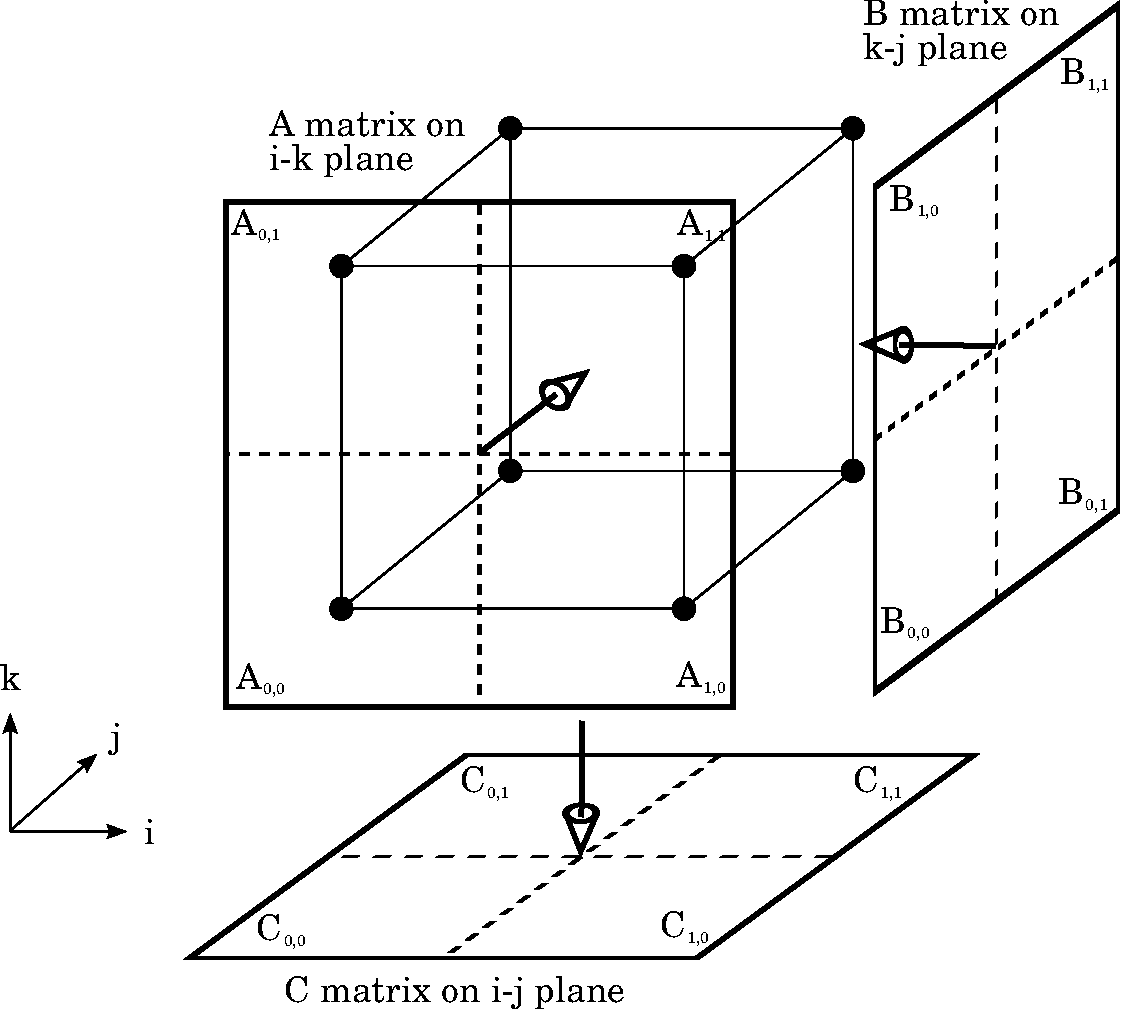
\includegraphics[width=0.8\textwidth]{images/dns.pdf}
    \caption{An overview of the DNS algorithm.  The A, B and C matrix planes show the scatter/gather operations while the orthogonal arrows show the broadcast/reduce operations.}
    \label{fig:all_results}
\end{figure}

\subsubsection{Local memory usage}

Since a cost efficient formulation of the DNS algorithm uses $p < n$, each
processor gets an $(n/q \times n/q)$ submatrix, where $q = \sqrt[3]{p}$, for
each matrix $A$ and $B$.  It also stores the output matrix $C$.  Therefore the
local storage requirements for the DNS algorithm is $$3 \cdot {\left(\frac{n}{\sqrt[3]{p}}\right)}^2 = O\left(\frac{n^2}{p^{2/3}}\right)$$ at each
processor.

\subsubsection{Parallel Computation Time (Local Computations)}

Each processor has to serial multiply its submatrices, which are square matrices with dimension $ n/\sqrt[3]{p}$, therefore the
overall time spent for local computations is 
$$T_{{comp}} = \left(\frac{n}{\sqrt[3]{p}}\right)^3 = \frac{n^3}{p}$$

\subsubsection{Parallel Communication Time}

The parallel communication time comes from the following operations:
\begin{itemize}
  \item Two scatter operations for matrices A and B on a 2D mesh, with each mesh dimension having $q = \sqrt[3]{p}$ processors, 
  and the message size $m = (n/q)^2 = n^2/p^{2/3}$.
	\begin{eqnarray*}
  			T_{{scatter},{mesh}} &=& 2 \left[ t_s \log{q} + t_w  m (q-1) \right] \\
  								 &=& 2 \left[ t_s \log{\sqrt[3]{p}} + t_w \left( \frac{n}{\sqrt[3]{p}} \right)^2 (\sqrt[3]{p} - 1) \right] \\
   								 &=& 2 \left[ \frac{1}{3} t_s  \log{p} + t_w  \frac{n^2}{\sqrt[3]{p}} - t_w \frac{n^2}{\sqrt[3]{p}^2}  \right]		 
  	\end{eqnarray*}
  \item Two one-to-all broadcast on a ring with $q = \sqrt[3]{p}$ processors and message size $m = (n/q)^2 = n^2/p^{2/3}$.
  	\begin{eqnarray*}
  		 T_{{broadcast},{ring}} &=& 2 (t_s + t_w\cdot m) \log{q} \\
  		 						&=& \frac{2}{3} \left(t_s + t_w \frac{n^2}{p^{2/3}}\right) \log{p} \\
  		 						&=& \frac{2}{3} \left( t_s \log{p} + t_w \log{p} \frac{n^2}{p^{2/3}} \right)
  	\end{eqnarray*}
  \item Reduce on a ring with $q = \sqrt[3]{p}$ processors.  This time is identical to the one-to-all broadcast.
  \item Gather the final matrix, on a 2D mesh with each dimension having $q = \sqrt[3]{p}$ processors.  This time is identical 
  to the time it takes to do one scatter operation, and can be easily derived from the scatter formula above.
\end{itemize}

Therefore our total communication time is:
\begin{eqnarray*}
T_{{comm}} &=& T_{{scatter},{gather}} + T_{{broadcast},{reduce}} \\
		   &=& 3 \left( \frac{1}{3} t_s  \log{p} + t_w  \frac{n^2}{\sqrt[3]{p}} - t_w \frac{n^2}{\sqrt[3]{p}^2}  \right) +
		     \frac{3}{3} \left( t_s \log{p} + t_w \log{p} \frac{n^2}{p^{2/3}} \right) \\
		   &=& 2 t_s \log{p} + 3 t_w \left( \frac{n^2}{{p}^{1/3}} \right) + t_w \frac{n^2}{p^{2/3}} (\log{p} - 3)
\end{eqnarray*}

\subsubsection{Parallel Run Time}

Using the formula $T_p = T_{{comp}} + T_{{comm}}$ we get that 
\begin{eqnarray*}
T_p &=& \frac{n^3}{p} + 2 t_s \log{p} + 3 t_w \left( \frac{n^2}{{p}^{1/3}} \right) + t_w \frac{n^2}{p^{2/3}} (\log{p} - 3)
\end{eqnarray*}

\subsubsection{Speedup}

\begin{eqnarray*}
S &=& \frac{T_s}{T_p} \\
  &=& \frac{n^3}{\frac{n^3}{p} + 2 t_s \log{p} + 3 t_w \left( \frac{n^2}{{p}^{1/3}} \right) + t_w \frac{n^2}{p^{2/3}} (\log{p} - 3)} \\
  &=& \frac{1}{ \frac{1}{p} + 2 t_s \frac{\log{p}}{n^3} + \frac{3 t_w}{p^{1/3} n} + \frac{t_w (\log{p} - 3)}{p^{2/3} n} } \\
  &=& \frac{p}{   1 + 2 t_s \frac{ p \log{p} }{ n^3 } + 3 t_w \frac{p^{2/3}}{n} + t_w \frac{p^{1/3} (\log{p} - 3)}{n}      }
\end{eqnarray*}

It can be seen from the equation that as the matrix increases in size, the speedup tends to become linear.

\subsubsection{Cost}

\begin{eqnarray*}
C &=& p T_p \\
  &=& n^3 + 2 t_s p \log{p} + 3 t_w p^{2/3} n^2 + t_w p^{1/3} n^2 (\log{p} - 3)
\end{eqnarray*}

\subsubsection{Efficiency}

\begin{eqnarray*}
E &=& \frac{T_s}{p T_p} = \frac{S}{p} \\
  &=& \frac{1}{   1 + 2 t_s \frac{ p \log{p} }{ n^3 } + 3 t_w \frac{p^{2/3}}{n} + t_w \frac{p^{1/3} (\log{p} - 3)}{n} } \\
\end{eqnarray*}

\subsubsection{Cost optimality and Isoefficiency function}

In order for our algorithm to be cost optimal with regards to the serial formulation, the efficiency must remain constant as the
number of processors and the size of the matrices being multiplied increase.  In our case the efficiency is:

\begin{eqnarray*}
E &=& \frac{1}{   1 + 2 t_s \frac{ p \log{p} }{ n^3 } + 3 t_w \frac{p^{2/3}}{n} + t_w \frac{p^{1/3} (\log{p} - 3)}{n} }
\end{eqnarray*}

and asymptotically the $p^{2/3}/n$ term dominates all the other terms in the denominator, and therefore, in order for the algorithm to be cost 
optimal $$O(n) = O(p^{2/3})$$

For our problem of matrix multiplication, $W = n^3$, so therefore the isoefficiency function becomes:
$$W = O(p^2)$$

\subsection{LU Decomposition using 2D paritioning (optimized)}

As part of our effort to reduce the running time of the overall algorithm
(matrix multiplication plus computing the determininat) we updated our LU-2D
decomposition algorithm from our implementation in Assignment 02 by removing all
broadcast communications and opting for pipelined communication.  This greatly
reduced the running time of our algorithm.

\subsection{LU Decomposition using 1D partitioning (new)}


The DNS algorithm requires a perfect cube number of processors ($p = q^3$) while
the LU decomposition using a 2D mesh requires a perfect square number of
processors.  Because of the limitations on ARGO, the DNS algorithm can only run
with 8 processes and this is not compatible with our 2D LU decomposition
algorithm.

In order resolve this problem, we also implemented LU Decomposition using 1D
paritioning on a ring topology.  The assignment of the rows were done in a
cyclic fashion in order to balance the workload over all the processors as the
decomposition progresses.

\subsection{Strassen's Matrix Multiplication (serial formulation)}

In order to further improve performance, we implemented the serial version of
Strassen's matrix multiplication algorithm, which we run instead of the naive
matrix multiplication at each node when multiplying the sub matrices distributed
to each node.  The main benefit of Strassen's matrix multiplication is that the
runtime of the algorithm is $\approx O(N^{2.807})$, allowing us to save time
over the standard matrix multiplication with runtime of $O(N^3)$ when dealing
with large matrices .

\section{Parameter Ranges}

Each of the programs were tested with $n \times n$ matrix input sizes of $$n =
\{ 16, 64, 256, 512, 1024, 2048, 4096 \}$$ with powers of $$k=\{ 2, 4, 8,
16 \}$$ and with processors $p$ and cores $c$ ranging from $$(p,c) = \{ (1,4),
(2,2), (4,1), (4,4), (8,2) \}$$

The DNS algorithm can only be run with a perfect cube number of processes, and
on ARGO that limits us to 8 processes.

\section{Results}


\begin{table}[h]
	\centering
\begin{tabular}{|rr|r|r|r|r|r|r|}
\hline
n & \backslashbox{k}{p,c} & (1,1) & (1,4) & (2,2) & (4,1) & (4,4) & (8,2) \\
\hline
\multirow{2}{*}{16} & 2
& 0.000 & 0.126 & 0.128 & 0.090 & 0.140 & 3.136 \\
& 4
& 0.000 & 0.124 & 0.131 & 0.090 & 0.262 & 0.221 \\
& 8
& 0.001 & 0.126 & 0.130 & 0.093 & 0.185 & 0.187 \\
& 16
& 0.001 & 0.128 & 0.133 & 0.137 & 0.194 & 0.204 \\
\hline
\multirow{2}{*}{64} & 2
& 0.005 & 0.051 & 0.081 & 0.084 & 0.147 & 1.629 \\
& 4
& 0.011 & 0.058 & 0.058 & 0.066 & 0.198 & 0.122 \\
& 8
& 0.022 & 0.060 & 0.103 & 0.076 & 0.159 & 0.258 \\
& 16
& 0.044 & 0.072 & 0.116 & 0.095 & 0.134 & 0.141 \\
\hline
\multirow{2}{*}{256} & 2
& 0.318 & 0.218 & 0.419 & 0.210 & 0.224 & 0.196 \\
& 4
& 0.751 & 0.358 & 0.271 & 0.410 & 0.415 & 0.516 \\
& 8
& 1.858 & 0.685 & 0.613 & 0.566 & 2.561 & 2.692 \\
& 16
& 3.159 & 1.340 & 0.836 & 1.489 & 1.362 & 3.282 \\
\hline
\multirow{2}{*}{512} & 2
& 10.334 & 1.453 & 1.335 & 1.197 & 0.734 & 0.973 \\
& 4
& 29.127 & 4.531 & 1.977 & 2.947 & 1.079 & 1.840 \\
& 8
& 67.746 & 6.397 & 5.945 & 5.085 & 4.092 & 2.876 \\
& 16
& 145.336 & 15.241 & 11.347 & 12.187 & 3.827 & 5.708 \\
\hline
\multirow{2}{*}{1024} & 2
& 89.888 & 56.628 & 25.703 & 23.241 & 5.652 & 4.704 \\
& 4
& 250.687 & 162.152 & 74.140 & 61.505 & 13.904 & 10.239 \\
& 8
& 577.623 & 372.094 & 167.273 & 139.389 & 20.270 & 19.932 \\
& 16
& 1225.960 & 783.157 & 440.774 & 452.780 & 48.695 & 28.922 \\
\hline
\multirow{2}{*}{4096} & 2
& 6107.030 & 4094.002 & - & - & - & - \\
& 4
& - & - & - & - & - & - \\
& 8
& - & - & - & - & - & - \\
& 16
& - & - & - & - & - & - \\
\hline
\end{tabular}
\caption{Total runtime (in seconds) for the Cannon formulation.}
	\label{tab:cannontotal}
\end{table}
\begin{table}[h]
	\centering
\begin{tabular}{|rr|r|r|r|r|r|r|}
\hline
n & \backslashbox{k}{p,c} & (1,1) & (1,4) & (2,2) & (4,1) & (4,4) & (8,2) \\
\hline
\multirow{2}{*}{64} & 2
& 0.005 & 0.052 & 0.056 & 0.063 & 0.155 & 0.200 \\
& 4
& 0.011 & 0.053 & 0.099 & 0.066 & 0.119 & 0.115 \\
& 8
& 0.022 & 0.066 & 0.103 & 0.073 & 0.162 & 0.210 \\
& 16
& 0.044 & 0.070 & 0.116 & 0.131 & 0.131 & 0.186 \\
\hline
\multirow{2}{*}{256} & 2
& 0.321 & 0.232 & 0.210 & 0.240 & 0.171 & 0.220 \\
& 4
& 1.087 & 0.358 & 0.269 & 0.530 & 0.328 & 0.261 \\
& 8
& 1.514 & 0.690 & 0.497 & 0.757 & 1.609 & 0.831 \\
& 16
& 3.197 & 1.342 & 0.835 & 1.499 & 1.625 & 1.714 \\
\hline
\multirow{2}{*}{512} & 2
& 10.400 & 1.405 & 1.438 & 0.970 & 0.766 & 3.669 \\
& 4
& 29.507 & 4.594 & 1.707 & 4.082 & 1.108 & - \\
& 8
& 66.953 & 7.630 & 3.462 & 11.437 & 2.145 & - \\
& 16
& 142.902 & 24.803 & 6.970 & 7.600 & 4.226 & - \\
\hline
\multirow{2}{*}{1024} & 2
& 88.914 & 60.955 & 26.306 & 22.502 & 7.889 & - \\
& 4
& 251.556 & 158.169 & 73.175 & 61.663 & 10.205 & - \\
& 8
& 579.038 & 399.187 & 168.147 & 139.759 & - & - \\
& 16
& 1227.902 & 785.612 & 594.923 & 312.681 & - & - \\
\hline
\end{tabular}
\caption{Total runtime (in seconds) for the cannon -s formulation.}
	\label{tab:cannon -stotal}
\end{table}
\begin{table}[h]
	\centering
\begin{tabular}{|rr|r|r|r|}
\hline
n & \backslashbox{k}{p,c} & (2,4) & (4,2) & (8,1) \\
\hline
\multirow{2}{*}{16} & 2
& 0.046 & 0.108 & - \\
& 4
& 0.046 & 0.087 & 0.087 \\
& 8
& 0.008 & 0.090 & 0.091 \\
& 16
& 0.051 & 0.093 & 0.101 \\
\hline
\multirow{2}{*}{256} & 2
& 0.145 & 0.166 & 0.259 \\
& 4
& 0.230 & 0.239 & - \\
& 8
& 0.414 & 0.379 & - \\
& 16
& 0.790 & 0.658 & - \\
\hline
\multirow{2}{*}{512} & 2
& 0.850 & 0.692 & - \\
& 4
& 1.660 & 1.629 & - \\
& 8
& 3.475 & 2.541 & - \\
& 16
& 7.052 & 4.718 & - \\
\hline
\multirow{2}{*}{1024} & 2
& 28.547 & 16.090 & - \\
& 4
& 82.221 & 42.795 & - \\
& 8
& 186.681 & 92.067 & - \\
& 16
& 416.023 & 191.168 & - \\
\hline
\end{tabular}
\caption{Total runtime (in seconds) for the DNS formulation.}
	\label{tab:dnstotal}
\end{table}

\begin{table}[h]
	\centering
\begin{tabular}{|rr|r|r|r|r|r|r|}
\hline
n & \backslashbox{k}{p,c} & (1,1) & (1,4) & (2,2) & (4,1) & (4,4) & (8,2) \\
\hline
\multirow{2}{*}{16} & 2
& 0.000 & 0.000 & 0.001 & 0.001 & 0.043 & 0.045 \\
& 4
& 0.000 & 0.001 & 0.002 & 0.002 & 0.090 & 0.123 \\
& 8
& 0.000 & 0.002 & 0.003 & 0.004 & 0.090 & 0.090 \\
& 16
& 0.001 & 0.003 & 0.006 & 0.008 & 0.099 & 0.104 \\
\hline
\multirow{2}{*}{64} & 2
& 0.003 & 0.002 & 0.002 & 0.002 & 0.004 & 0.004 \\
& 4
& 0.008 & 0.007 & 0.004 & 0.007 & 0.007 & 0.009 \\
& 8
& 0.020 & 0.010 & 0.011 & 0.017 & 0.013 & 0.022 \\
& 16
& 0.042 & 0.021 & 0.022 & 0.036 & 0.024 & 0.029 \\
\hline
\multirow{2}{*}{256} & 2
& 0.207 & 0.084 & 0.221 & 0.058 & 0.029 & 0.029 \\
& 4
& 0.637 & 0.247 & 0.151 & 0.275 & 0.219 & 0.294 \\
& 8
& 1.744 & 0.573 & 0.484 & 0.429 & 0.762 & 0.927 \\
& 16
& 3.046 & 1.228 & 0.721 & 1.335 & 1.125 & 1.502 \\
\hline
\multirow{2}{*}{512} & 2
& 9.397 & 0.906 & 0.904 & 0.714 & 0.312 & 0.276 \\
& 4
& 28.190 & 3.959 & 1.581 & 2.325 & 0.715 & 1.279 \\
& 8
& 66.813 & 5.846 & 5.540 & 4.606 & 2.056 & 2.479 \\
& 16
& 144.412 & 14.686 & 10.916 & 11.691 & 3.478 & 5.297 \\
\hline
\multirow{2}{*}{1024} & 2
& 82.464 & 52.263 & 23.107 & 19.935 & 2.983 & 2.831 \\
& 4
& 243.280 & 157.828 & 71.323 & 58.715 & 12.290 & 5.662 \\
& 8
& 570.166 & 367.698 & 164.388 & 136.662 & 15.574 & 18.707 \\
& 16
& 1218.535 & 778.853 & 437.901 & 450.020 & 43.790 & 27.425 \\
\hline
\multirow{2}{*}{4096} & 2
& 5638.575 & 3836.591 & - & - & - & - \\
& 4
& - & - & - & - & - & - \\
& 8
& - & - & - & - & - & - \\
& 16
& - & - & - & - & - & - \\
\hline
\end{tabular}
\caption{Multiplication time (in seconds) for the Cannon formulation.}
	\label{tab:cannonmatrix multiplication}
\end{table}
\begin{table}[h]
	\centering
\begin{tabular}{|rr|r|r|r|r|r|r|}
\hline
n & \backslashbox{k}{p,c} & (1,1) & (1,4) & (2,2) & (4,1) & (4,4) & (8,2) \\
\hline
\multirow{2}{*}{64} & 2
& 0.003 & 0.002 & 0.002 & 0.003 & 0.005 & 0.006 \\
& 4
& 0.008 & 0.004 & 0.005 & 0.007 & 0.008 & 0.008 \\
& 8
& 0.019 & 0.015 & 0.009 & 0.015 & 0.014 & 0.015 \\
& 16
& 0.042 & 0.021 & 0.022 & 0.032 & 0.024 & 0.031 \\
\hline
\multirow{2}{*}{256} & 2
& 0.207 & 0.082 & 0.052 & 0.086 & 0.028 & 0.029 \\
& 4
& 0.976 & 0.246 & 0.147 & 0.377 & 0.074 & 0.097 \\
& 8
& 1.403 & 0.575 & 0.340 & 0.645 & 1.138 & 0.606 \\
& 16
& 3.084 & 1.227 & 0.719 & 1.381 & 1.237 & 1.536 \\
\hline
\multirow{2}{*}{512} & 2
& 9.467 & 0.852 & 1.018 & 0.466 & 0.381 & 0.316 \\
& 4
& 28.579 & 4.044 & 1.315 & 3.615 & 0.714 & - \\
& 8
& 66.009 & 7.075 & 3.079 & 10.959 & 1.742 & - \\
& 16
& 141.978 & 24.271 & 6.574 & 7.134 & 3.793 & - \\
\hline
\multirow{2}{*}{1024} & 2
& 81.466 & 56.414 & 23.572 & 19.728 & 6.080 & - \\
& 4
& 244.112 & 153.833 & 70.478 & 59.004 & 8.581 & - \\
& 8
& 571.581 & 394.572 & 165.391 & 137.077 & - & - \\
& 16
& 1220.521 & 781.152 & 590.637 & 310.024 & - & - \\
\hline
\end{tabular}
\caption{Multiplication time (in seconds) for the cannon -s formulation.}
	\label{tab:cannon -smatrix multiplication}
\end{table}
\begin{table}[h]
	\centering
\begin{tabular}{|rr|r|r|r|}
\hline
n & \backslashbox{k}{p,c} & (2,4) & (4,2) & (8,1) \\
\hline
\multirow{2}{*}{16} & 2
& 0.001 & 0.001 & - \\
& 4
& 0.001 & 0.002 & 0.002 \\
& 8
& 0.003 & 0.004 & 0.005 \\
& 16
& 0.007 & 0.008 & 0.014 \\
\hline
\multirow{2}{*}{256} & 2
& 0.052 & 0.040 & 0.043 \\
& 4
& 0.153 & 0.115 & - \\
& 8
& 0.340 & 0.255 & - \\
& 16
& 0.715 & 0.533 & - \\
\hline
\multirow{2}{*}{512} & 2
& 0.507 & 0.345 & - \\
& 4
& 1.318 & 1.263 & - \\
& 8
& 3.136 & 2.213 & - \\
& 16
& 6.657 & 4.376 & - \\
\hline
\multirow{2}{*}{1024} & 2
& 25.959 & 14.375 & - \\
& 4
& 79.734 & 41.052 & - \\
& 8
& 184.148 & 90.423 & - \\
& 16
& 413.434 & 189.660 & - \\
\hline
\end{tabular}
\caption{Multiplication time (in seconds) for the DNS formulation.}
	\label{tab:dnsmatrix multiplication}
\end{table}

\begin{table}[h]
	\centering
\begin{tabular}{|rr|r|r|r|r|r|r|}
\hline
n & \backslashbox{k}{p,c} & (1,1) & (1,4) & (2,2) & (4,1) & (4,4) & (8,2) \\
\hline
\multirow{2}{*}{16} & 2
& 0.000 & 0.123 & 0.124 & 0.085 & 0.083 & 0.083 \\
& 4
& 0.000 & 0.121 & 0.125 & 0.085 & 0.093 & 0.084 \\
& 8
& 0.000 & 0.121 & 0.124 & 0.085 & 0.084 & 0.085 \\
& 16
& 0.000 & 0.123 & 0.124 & 0.125 & 0.084 & 0.086 \\
\hline
\multirow{2}{*}{64} & 2
& 0.002 & 0.046 & 0.076 & 0.078 & 0.133 & 0.114 \\
& 4
& 0.002 & 0.047 & 0.050 & 0.054 & 0.179 & 0.098 \\
& 8
& 0.002 & 0.047 & 0.089 & 0.053 & 0.133 & 0.222 \\
& 16
& 0.002 & 0.047 & 0.091 & 0.054 & 0.096 & 0.098 \\
\hline
\multirow{2}{*}{256} & 2
& 0.102 & 0.122 & 0.132 & 0.133 & 0.171 & 0.135 \\
& 4
& 0.104 & 0.099 & 0.107 & 0.114 & 0.169 & 0.170 \\
& 8
& 0.105 & 0.099 & 0.112 & 0.118 & 0.150 & 0.133 \\
& 16
& 0.104 & 0.100 & 0.102 & 0.130 & 0.210 & 0.151 \\
\hline
\multirow{2}{*}{512} & 2
& 0.901 & 0.504 & 0.375 & 0.416 & 0.277 & 0.408 \\
& 4
& 0.902 & 0.529 & 0.345 & 0.554 & 0.273 & 0.277 \\
& 8
& 0.897 & 0.507 & 0.355 & 0.411 & 0.253 & 0.290 \\
& 16
& 0.889 & 0.511 & 0.374 & 0.407 & 0.276 & 0.312 \\
\hline
\multirow{2}{*}{1024} & 2
& 7.285 & 4.202 & 2.403 & 2.977 & 1.421 & 1.368 \\
& 4
& 7.268 & 4.161 & 2.589 & 2.549 & 1.388 & 1.260 \\
& 8
& 7.319 & 4.223 & 2.677 & 2.489 & 1.405 & 0.959 \\
& 16
& 7.279 & 4.112 & 2.675 & 2.494 & 1.430 & 1.222 \\
\hline
\multirow{2}{*}{4096} & 2
& 465.553 & 254.962 & - & - & - & - \\
& 4
& - & - & - & - & - & - \\
& 8
& - & - & - & - & - & - \\
& 16
& - & - & - & - & - & - \\
\hline
\end{tabular}
\caption{LU decomposition time (in seconds) for the Cannon formulation.}
	\label{tab:cannonLU}
\end{table}
\begin{table}[h]
	\centering
\begin{tabular}{|rr|r|r|r|r|r|r|}
\hline
n & \backslashbox{k}{p,c} & (1,1) & (1,4) & (2,2) & (4,1) & (4,4) & (8,2) \\
\hline
\multirow{2}{*}{64} & 2
& 0.002 & 0.046 & 0.050 & 0.055 & 0.100 & 0.182 \\
& 4
& 0.002 & 0.046 & 0.090 & 0.054 & 0.099 & 0.095 \\
& 8
& 0.002 & 0.048 & 0.090 & 0.053 & 0.135 & 0.181 \\
& 16
& 0.002 & 0.046 & 0.091 & 0.093 & 0.096 & 0.141 \\
\hline
\multirow{2}{*}{256} & 2
& 0.105 & 0.138 & 0.143 & 0.137 & 0.114 & 0.153 \\
& 4
& 0.103 & 0.100 & 0.108 & 0.135 & 0.228 & 0.127 \\
& 8
& 0.102 & 0.102 & 0.143 & 0.091 & 0.238 & 0.189 \\
& 16
& 0.104 & 0.103 & 0.102 & 0.099 & 0.150 & 0.148 \\
\hline
\multirow{2}{*}{512} & 2
& 0.899 & 0.510 & 0.371 & 0.434 & 0.289 & 0.267 \\
& 4
& 0.894 & 0.508 & 0.336 & 0.406 & 0.331 & - \\
& 8
& 0.909 & 0.512 & 0.334 & 0.412 & 0.325 & - \\
& 16
& 0.888 & 0.490 & 0.346 & 0.403 & 0.336 & - \\
\hline
\multirow{2}{*}{1024} & 2
& 7.310 & 4.377 & 2.526 & 2.536 & 1.373 & - \\
& 4
& 7.308 & 4.176 & 2.486 & 2.421 & 1.395 & - \\
& 8
& 7.318 & 4.447 & 2.546 & 2.447 & - & - \\
& 16
& 7.245 & 4.298 & 4.070 & 2.429 & - & - \\
\hline
\end{tabular}
\caption{LU decomposition time (in seconds) for the cannon -s formulation.}
	\label{tab:cannon -sLU}
\end{table}
\begin{table}[h]
	\centering
\begin{tabular}{|rr|r|r|r|}
\hline
n & \backslashbox{k}{p,c} & (2,4) & (4,2) & (8,1) \\
\hline
\multirow{2}{*}{16} & 2
& 0.045 & 0.107 & - \\
& 4
& 0.045 & 0.085 & 0.084 \\
& 8
& 0.005 & 0.085 & 0.086 \\
& 16
& 0.045 & 0.085 & 0.087 \\
\hline
\multirow{2}{*}{256} & 2
& 0.087 & 0.120 & 0.212 \\
& 4
& 0.069 & 0.120 & - \\
& 8
& 0.066 & 0.119 & - \\
& 16
& 0.067 & 0.121 & - \\
\hline
\multirow{2}{*}{512} & 2
& 0.310 & 0.329 & - \\
& 4
& 0.307 & 0.349 & - \\
& 8
& 0.306 & 0.311 & - \\
& 16
& 0.362 & 0.308 & - \\
\hline
\multirow{2}{*}{1024} & 2
& 2.459 & 1.644 & - \\
& 4
& 2.359 & 1.668 & - \\
& 8
& 2.399 & 1.572 & - \\
& 16
& 2.454 & 1.438 & - \\
\hline
\end{tabular}
\caption{LU decomposition time (in seconds) for the DNS formulation.}
	\label{tab:dnsLU}
\end{table}

\begin{table}[h]
	\centering
\begin{tabular}{|rr|r|r|r|r|r|r|r|r|r|r|r|r|}
\hline
 &  & \multicolumn{2}{c}{(1,1)} & \multicolumn{2}{c}{(1,4)} & \multicolumn{2}{c}{(2,2)} & \multicolumn{2}{c}{(4,1)} & \multicolumn{2}{c}{(4,4)} & \multicolumn{2}{c}{(8,2)} \\
n & \backslashbox{k}{p,c} & 1d & 2d & 1d & 2d & 1d & 2d & 1d & 2d & 1d & 2d & 1d & 2d \\
\hline
\multirow{2}{*}{64} & 2
& 0.005 & - & 0.051 & 1.551 & 0.081 & - & 0.084 & 1.456 & 0.147 & 0.403 & 1.629 & 0.335 \\
\hline
\multirow{2}{*}{256} & 2
& 0.318 & - & 0.218 & - & 0.419 & 9.697 & 0.210 & - & 0.224 & - & 0.196 & - \\
\hline
\multirow{2}{*}{512} & 2
& 10.334 & 16.583 & 1.453 & - & 1.335 & - & 1.197 & - & 0.734 & - & 0.973 & - \\
\hline
\multirow{2}{*}{1024} & 2
& 89.888 & 133.654 & 56.628 & - & 25.703 & - & 23.241 & - & 5.652 & - & 4.704 & - \\
\hline
\end{tabular}
\caption{Total runtime (in seconds) for the Cannon formulation with 1D and 2D LU decomposition.}
	\label{tab:lucompare_total}
\end{table}

\begin{table}[h]
	\centering
\begin{tabular}{|rr|r|r|r|r|r|r|r|r|r|r|r|r|}
\hline
 &  & \multicolumn{2}{c}{(1,1)} & \multicolumn{2}{c}{(1,4)} & \multicolumn{2}{c}{(2,2)} & \multicolumn{2}{c}{(4,1)} & \multicolumn{2}{c}{(4,4)} & \multicolumn{2}{c}{(8,2)} \\
n & \backslashbox{k}{p,c} & 1d & 2d & 1d & 2d & 1d & 2d & 1d & 2d & 1d & 2d & 1d & 2d \\
\hline
\multirow{2}{*}{64} & 2
& 0.002 & - & 0.046 & 1.547 & 0.076 & - & 0.078 & 1.443 & 0.133 & 0.392 & 0.114 & 0.319 \\
\hline
\multirow{2}{*}{256} & 2
& 0.102 & - & 0.122 & - & 0.132 & 9.624 & 0.133 & - & 0.171 & - & 0.135 & - \\
\hline
\multirow{2}{*}{512} & 2
& 0.901 & 6.830 & 0.504 & - & 0.375 & - & 0.416 & - & 0.277 & - & 0.408 & - \\
\hline
\multirow{2}{*}{1024} & 2
& 7.285 & 52.065 & 4.202 & - & 2.403 & - & 2.977 & - & 1.421 & - & 1.368 & - \\
\hline
\end{tabular}
\caption{LU decomposition time (in seconds) for the Cannon formulation with 1D and 2D LU decomposition.}
	\label{tab:lucompare_LU}
\end{table}




\section{Analysis}

We applied Cannon's parallelization to two different matrix multiplication algorithms: the naive one, which is $O(n^3)$, and Strassen's, which is $O(n^{2.807})$. The communication overhead is exactly the same, but Strassen's computation time is $t_{{mult}} \cdot n^{2.807} \cdot  p^{-0.9035}$, compared to $t_{mult} \cdot n^3 / p$: therefore, the version using Strassen's has a better runtime. However, its isoefficiency function is worse: $k \cdot p^{3.3587}$ compared to $k \cdot p^3$.

It is difficult to compare Cannon and DNS directly, since the former algorithm requires a number of processors
 that is a square number, while the latter requires a cube. The smallest number of processors that would satisfy both is $2^6 = 64$, but we do not have
 that many processors available on Argo. However, by interpolating the measurements, DNS does not appear to be faster than Cannon's.

Our version of LU decomposition from assignment 2 required a square grid, and thus was not directly compatible with DNS. We implemented a new version with
1D decomposition, which is much faster due to improved pipelining.

Strassen's algorithm barely edges out the naive algorithm in our tests; we would need larger matrices to see a significant difference.


% \begin{figure}
% 	\centering
% 	\includegraphics[width=0.8\textwidth]{images/r-lu}
%     \caption{Runtimes of LU without pivoting using MPI\_Send and MPI\_Recv.}
%     \label{fig:lu_results}
% \end{figure}
% 
% \begin{figure}
% 	\centering
% 	\includegraphics[width=0.8\textwidth]{images/r-lub}
%     \caption{Runtimes of LU without pivoting using MPI\_BCast.}
%     \label{fig:lub_results}
% \end{figure}
% 
% \begin{figure}
% 	\centering
% 	\includegraphics[width=0.8\textwidth]{images/r-lubp}
%     \caption{Runtimes of LU with pivoting using MPI\_BCast.}
%     \label{fig:lubp_results}
% \end{figure}
% 
% \begin{figure}
% 	\centering
% 	\includegraphics[width=0.8\textwidth]{images/r-all}
%     \caption{Comparison of all algorithm with $n=16$.}
%     \label{fig:all_results}
% \end{figure}

%\section{Lessons}

\newpage
~

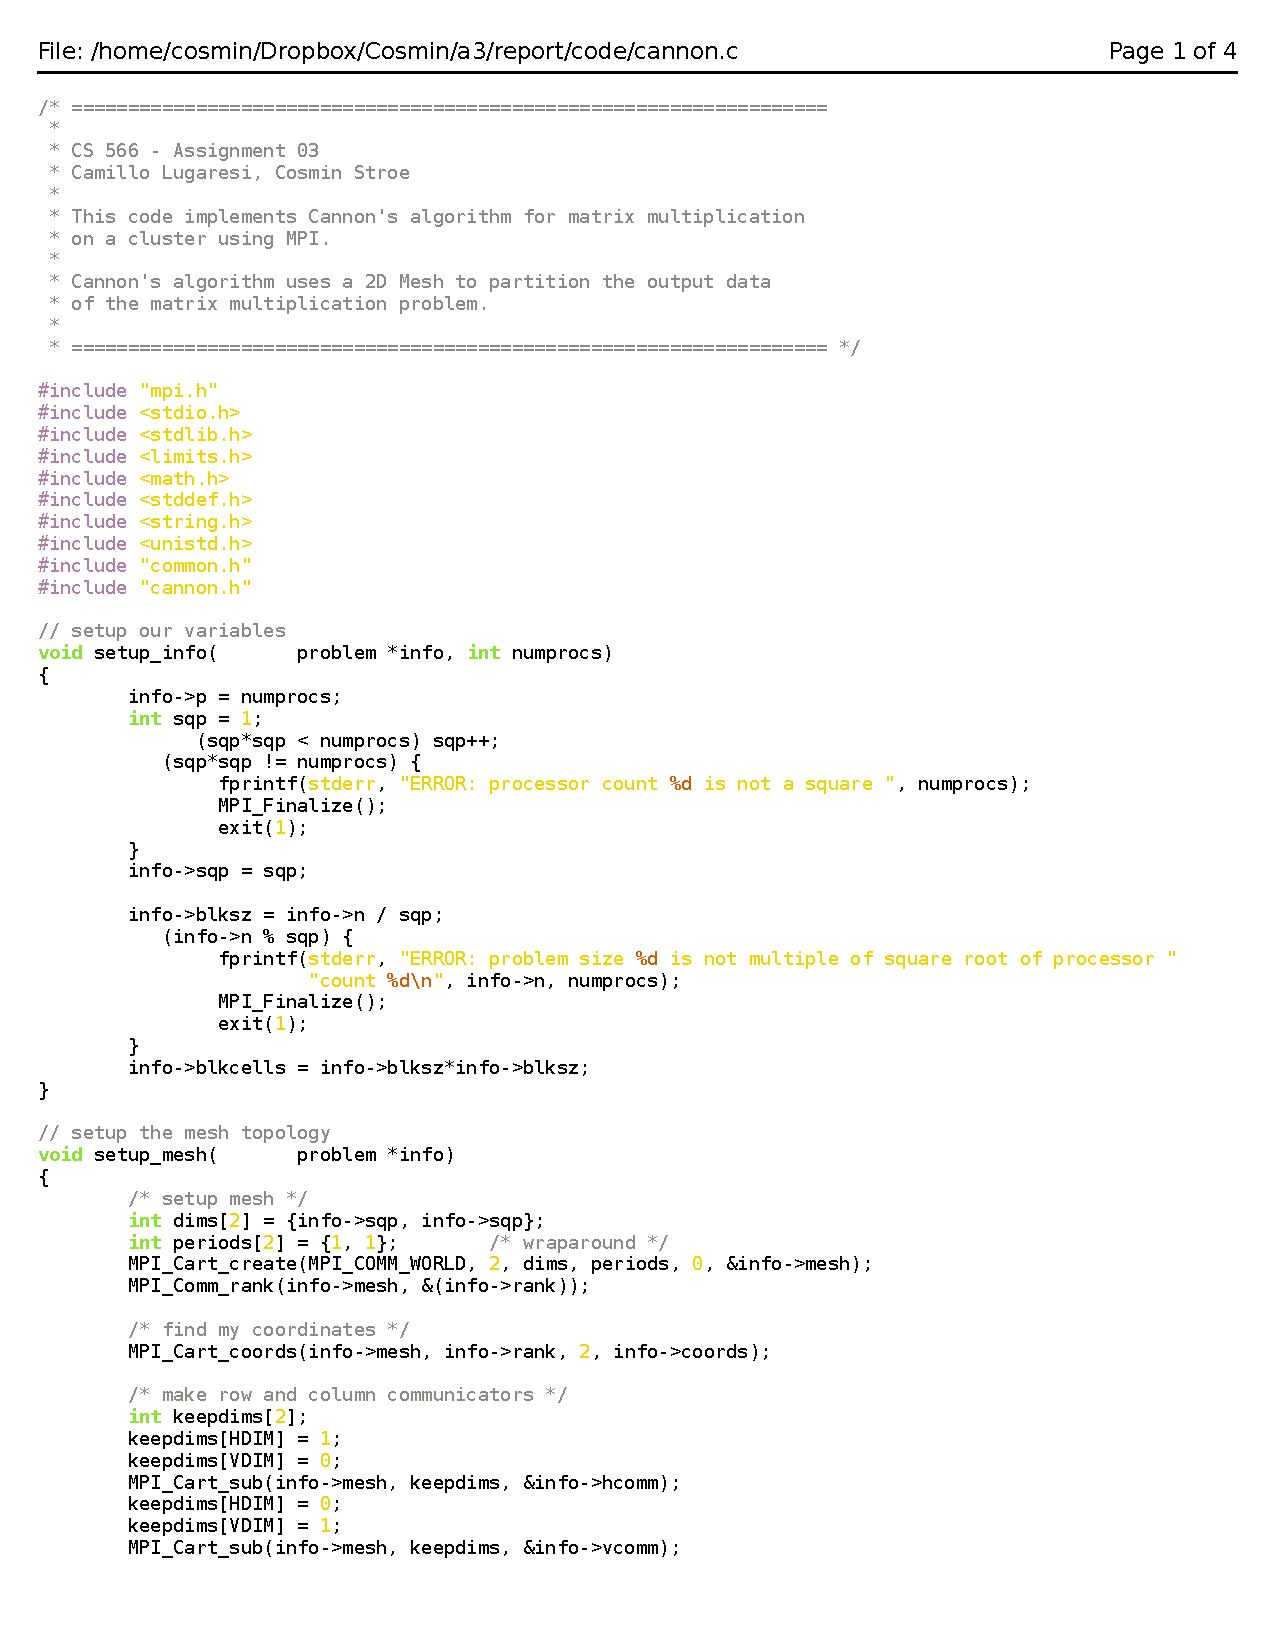
\includepdf[pages={-}]{code/pdf/cannon-c.pdf}
% 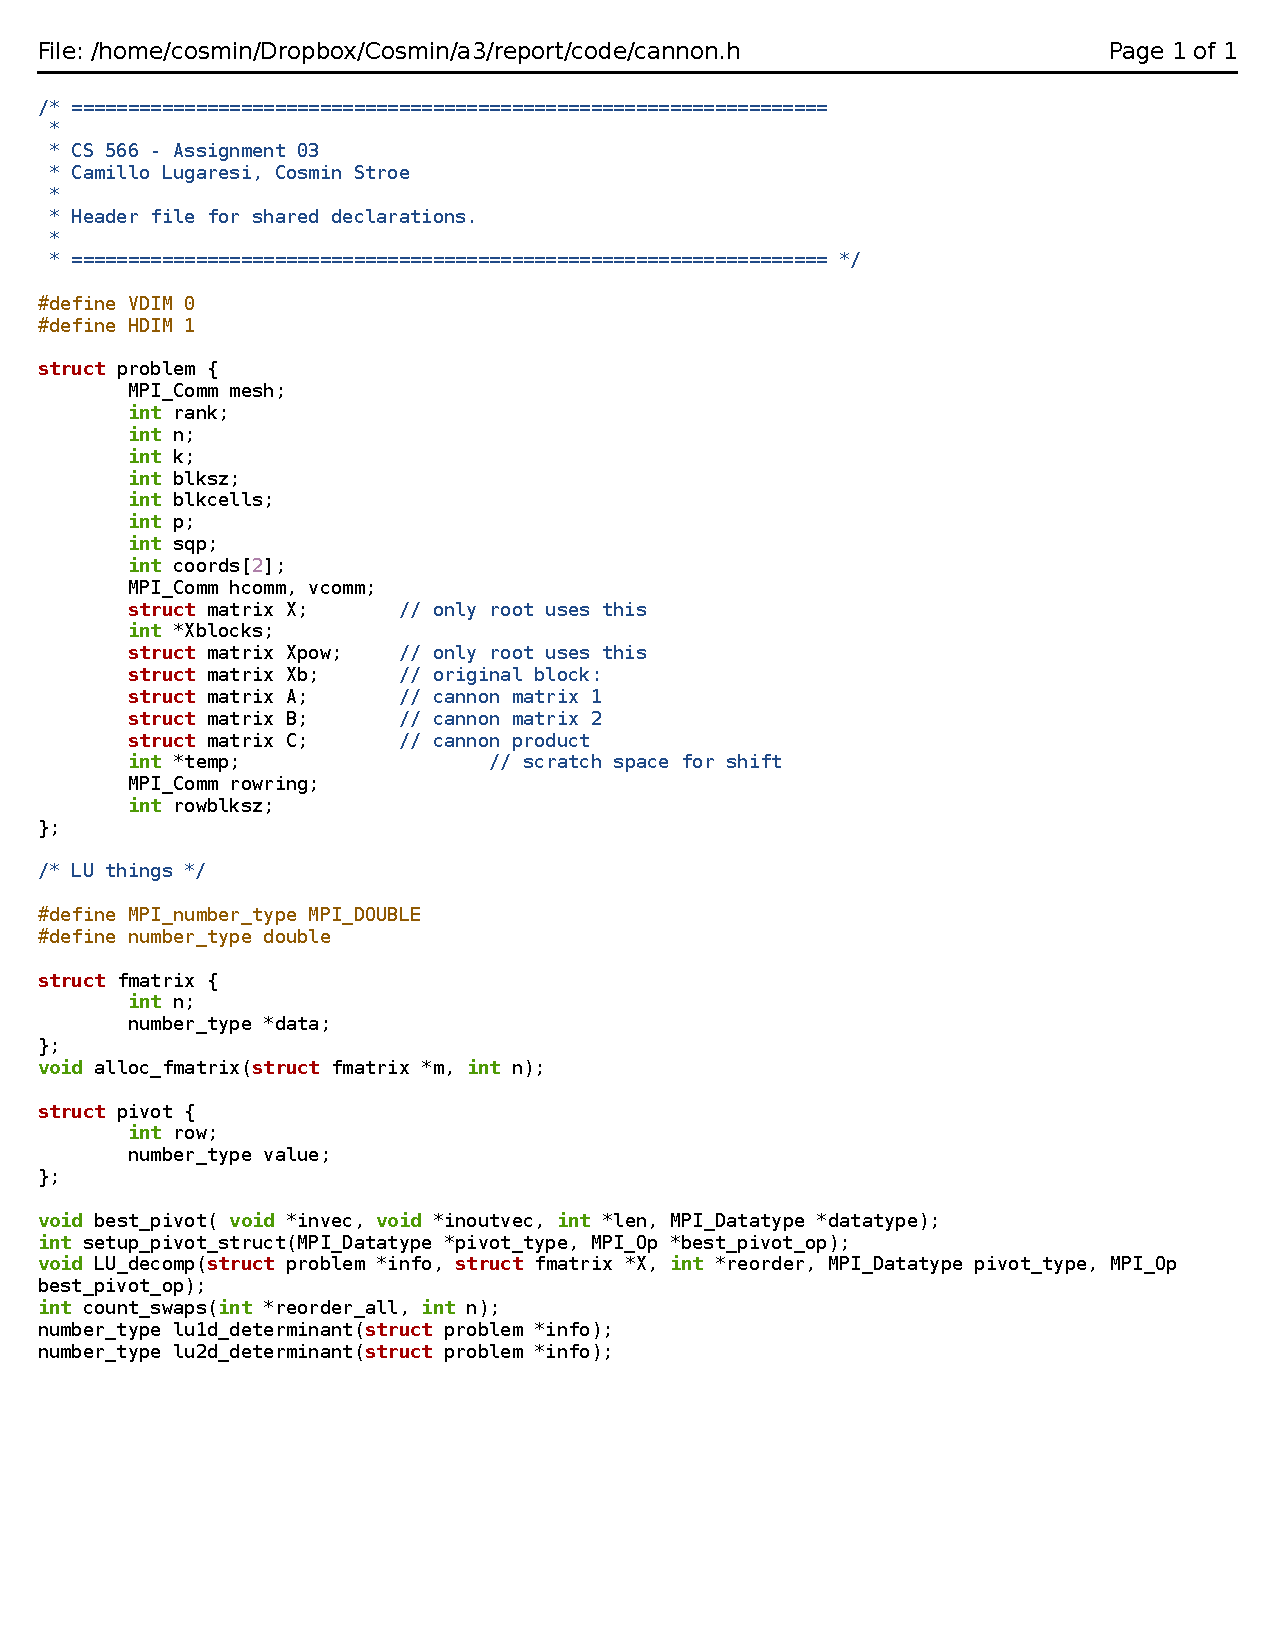
\includepdf[pages=-]{code/pdf/cannon-h.pdf}
% 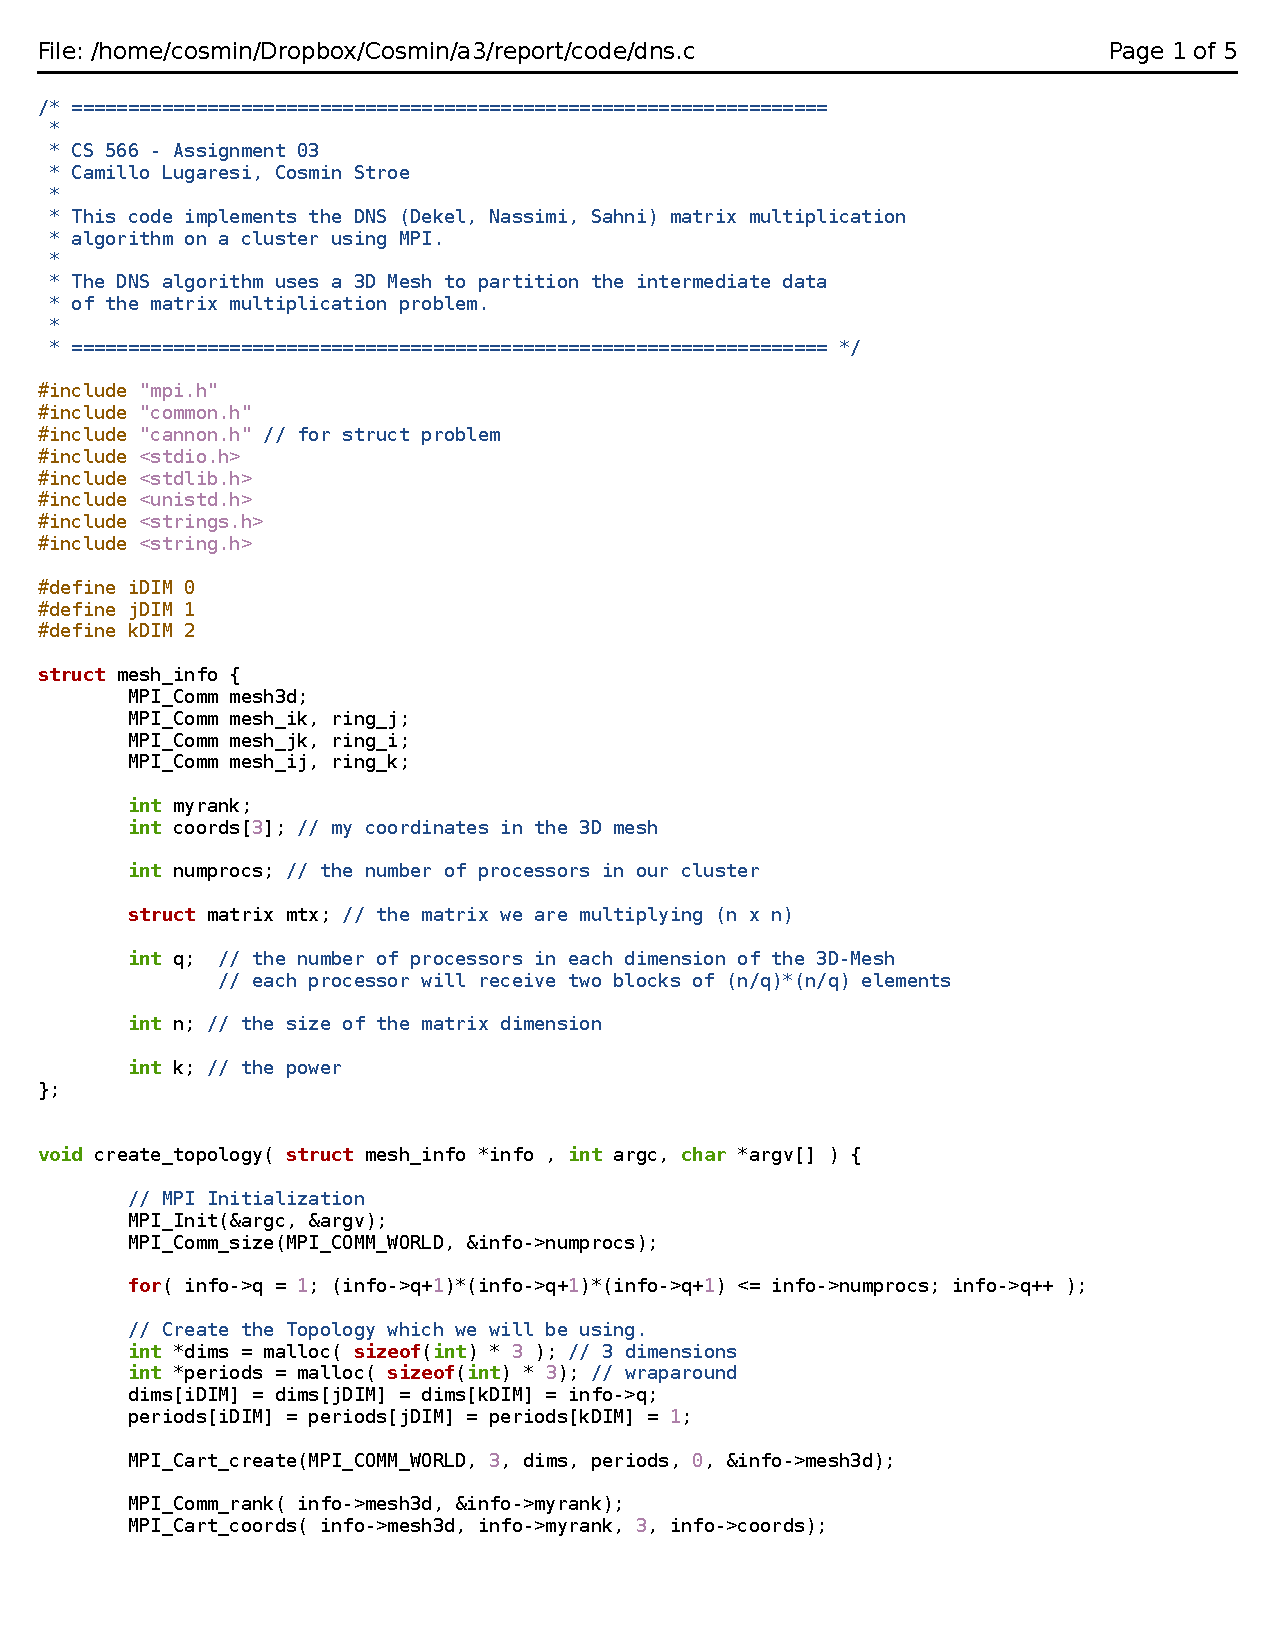
\includepdf[pages=-]{code/pdf/dns-c.pdf}
% 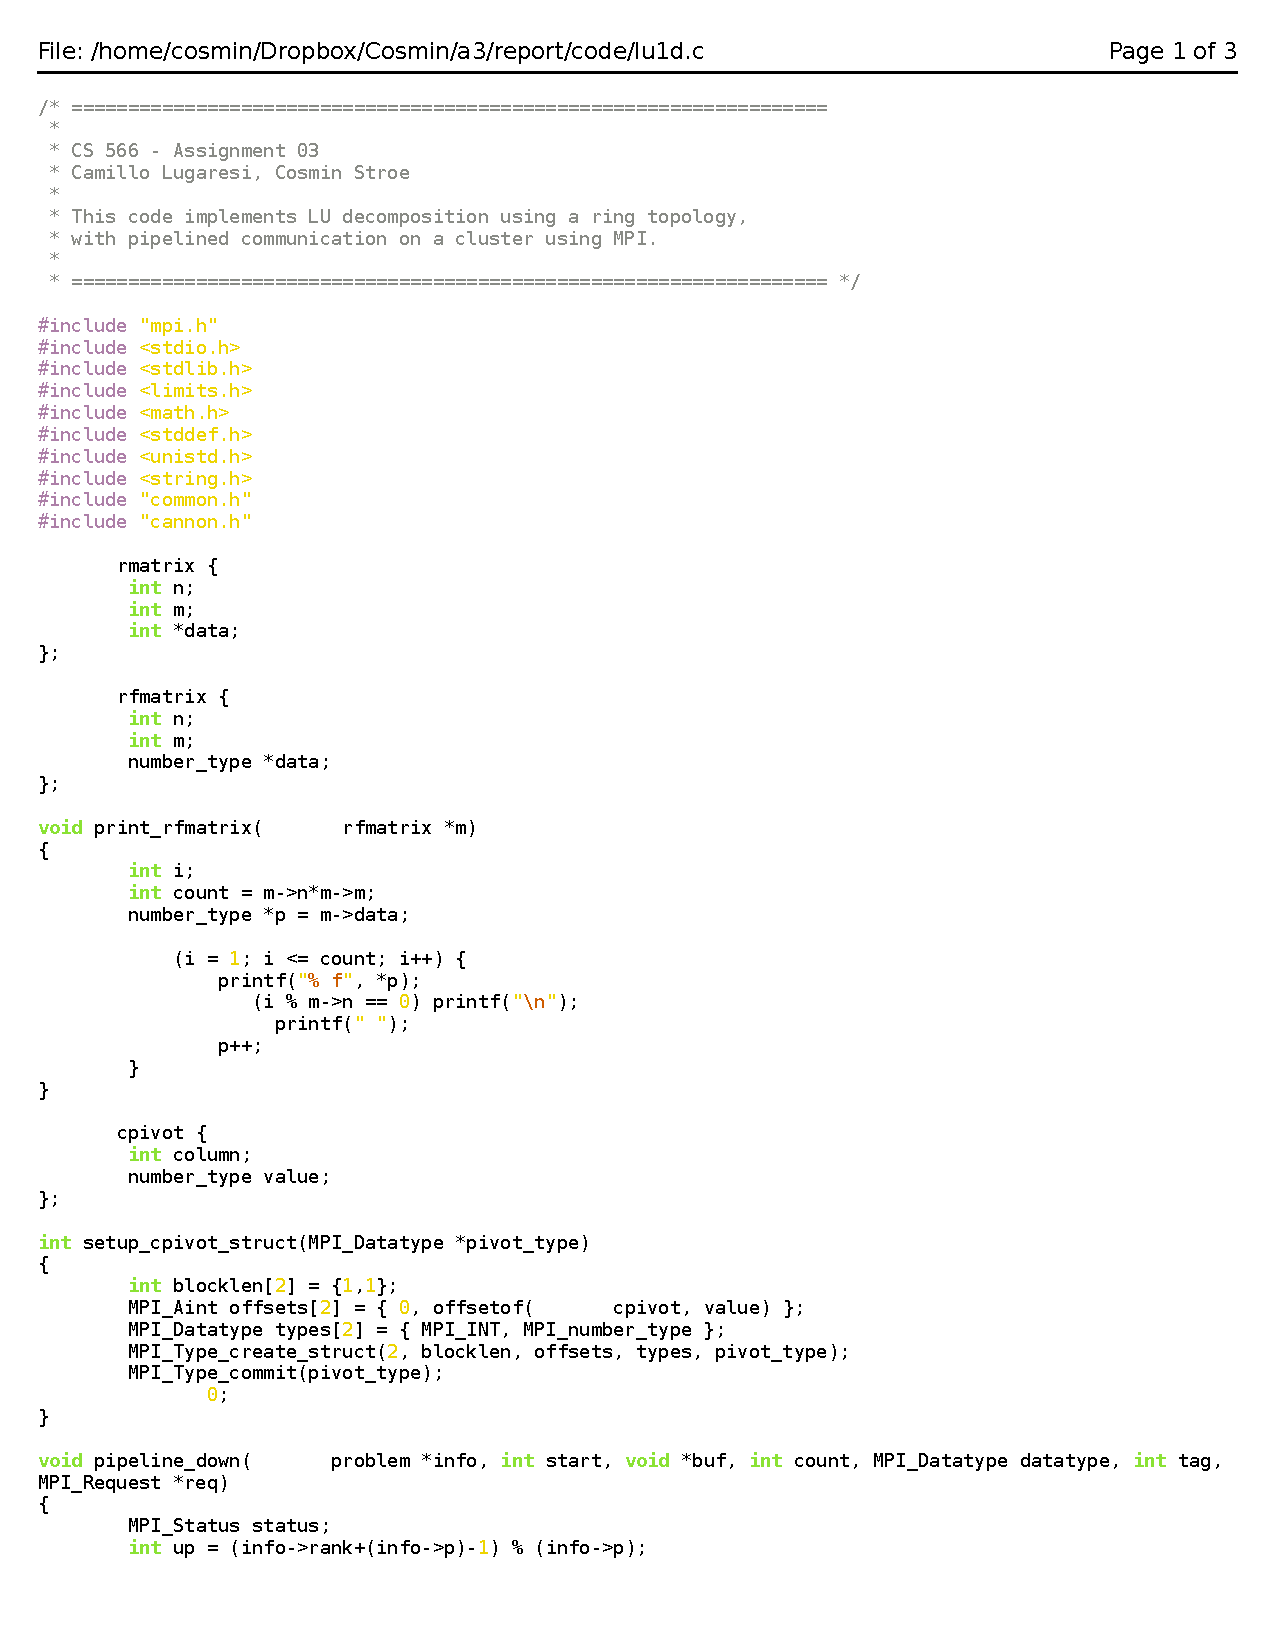
\includepdf[pages=-]{code/pdf/lu1d-c.pdf}
% 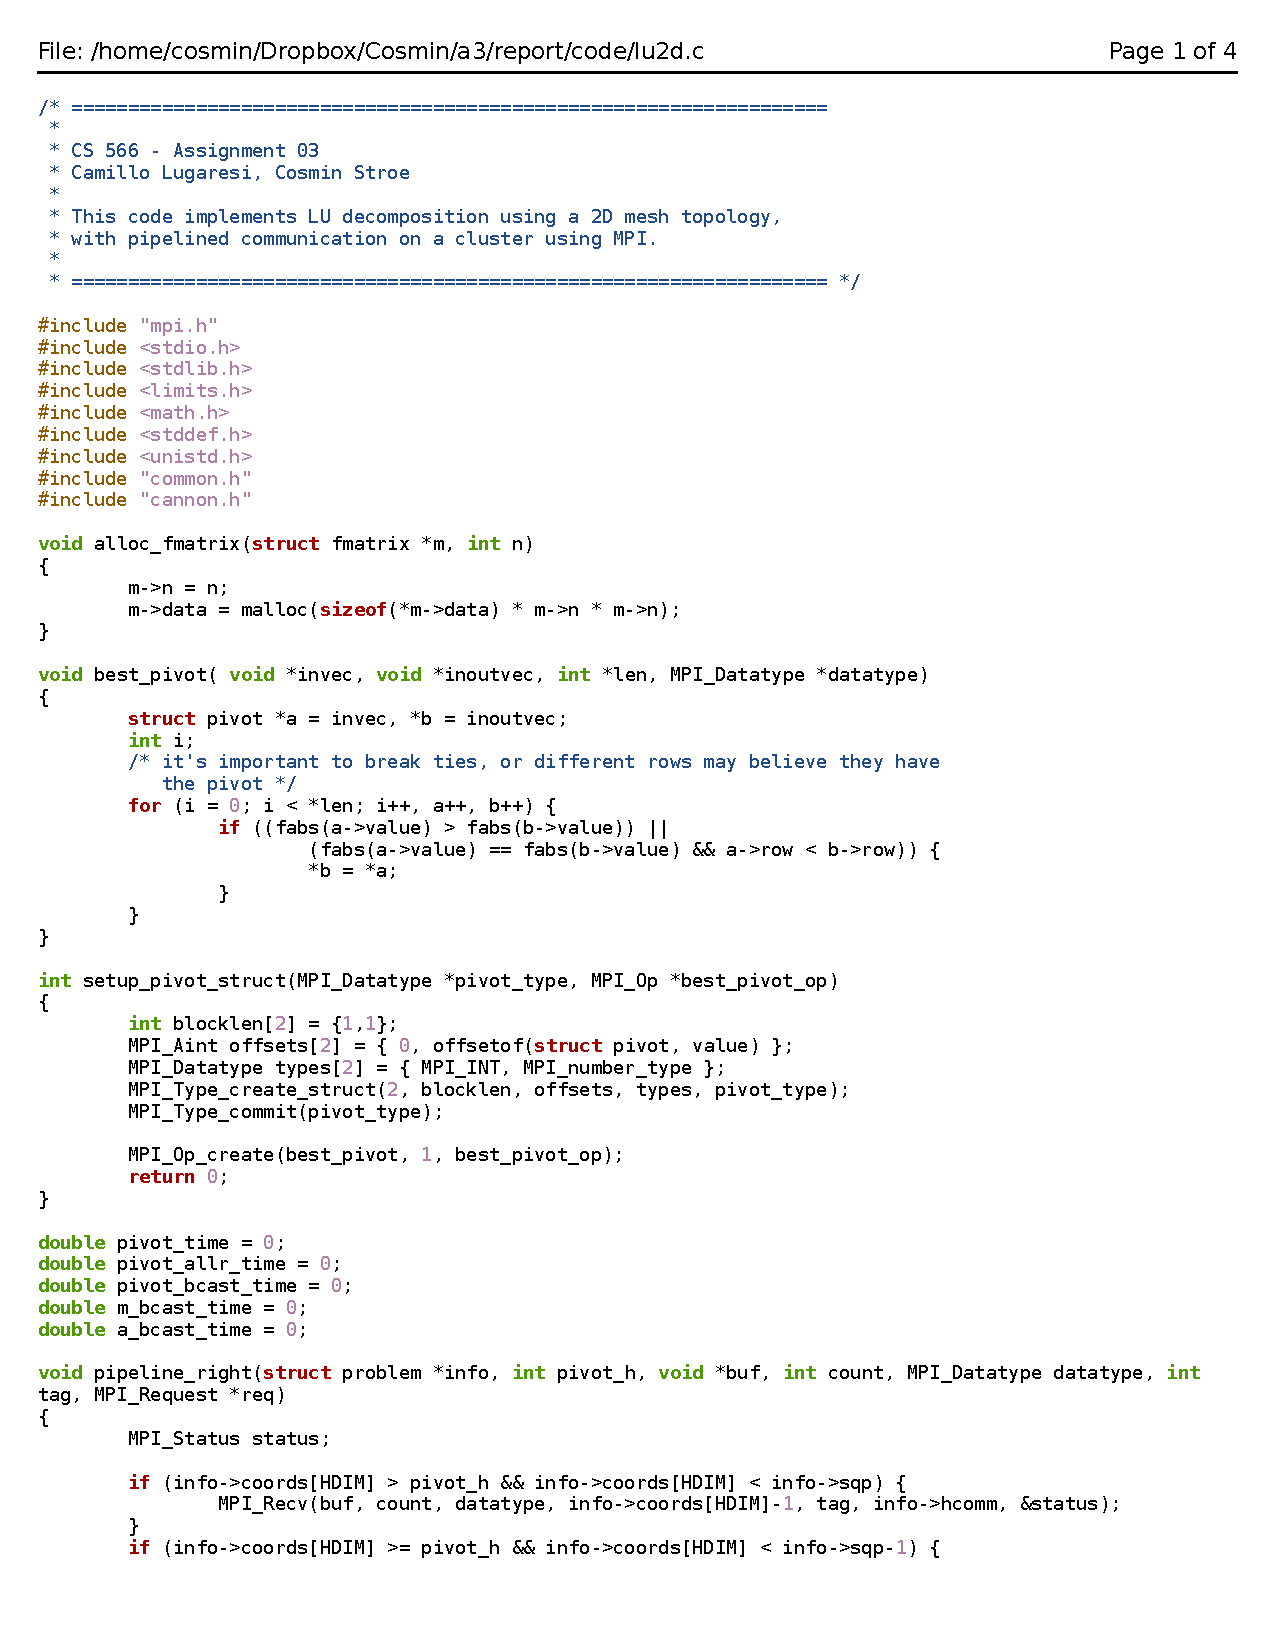
\includepdf[pages=-]{code/pdf/lu2d-c.pdf}
% 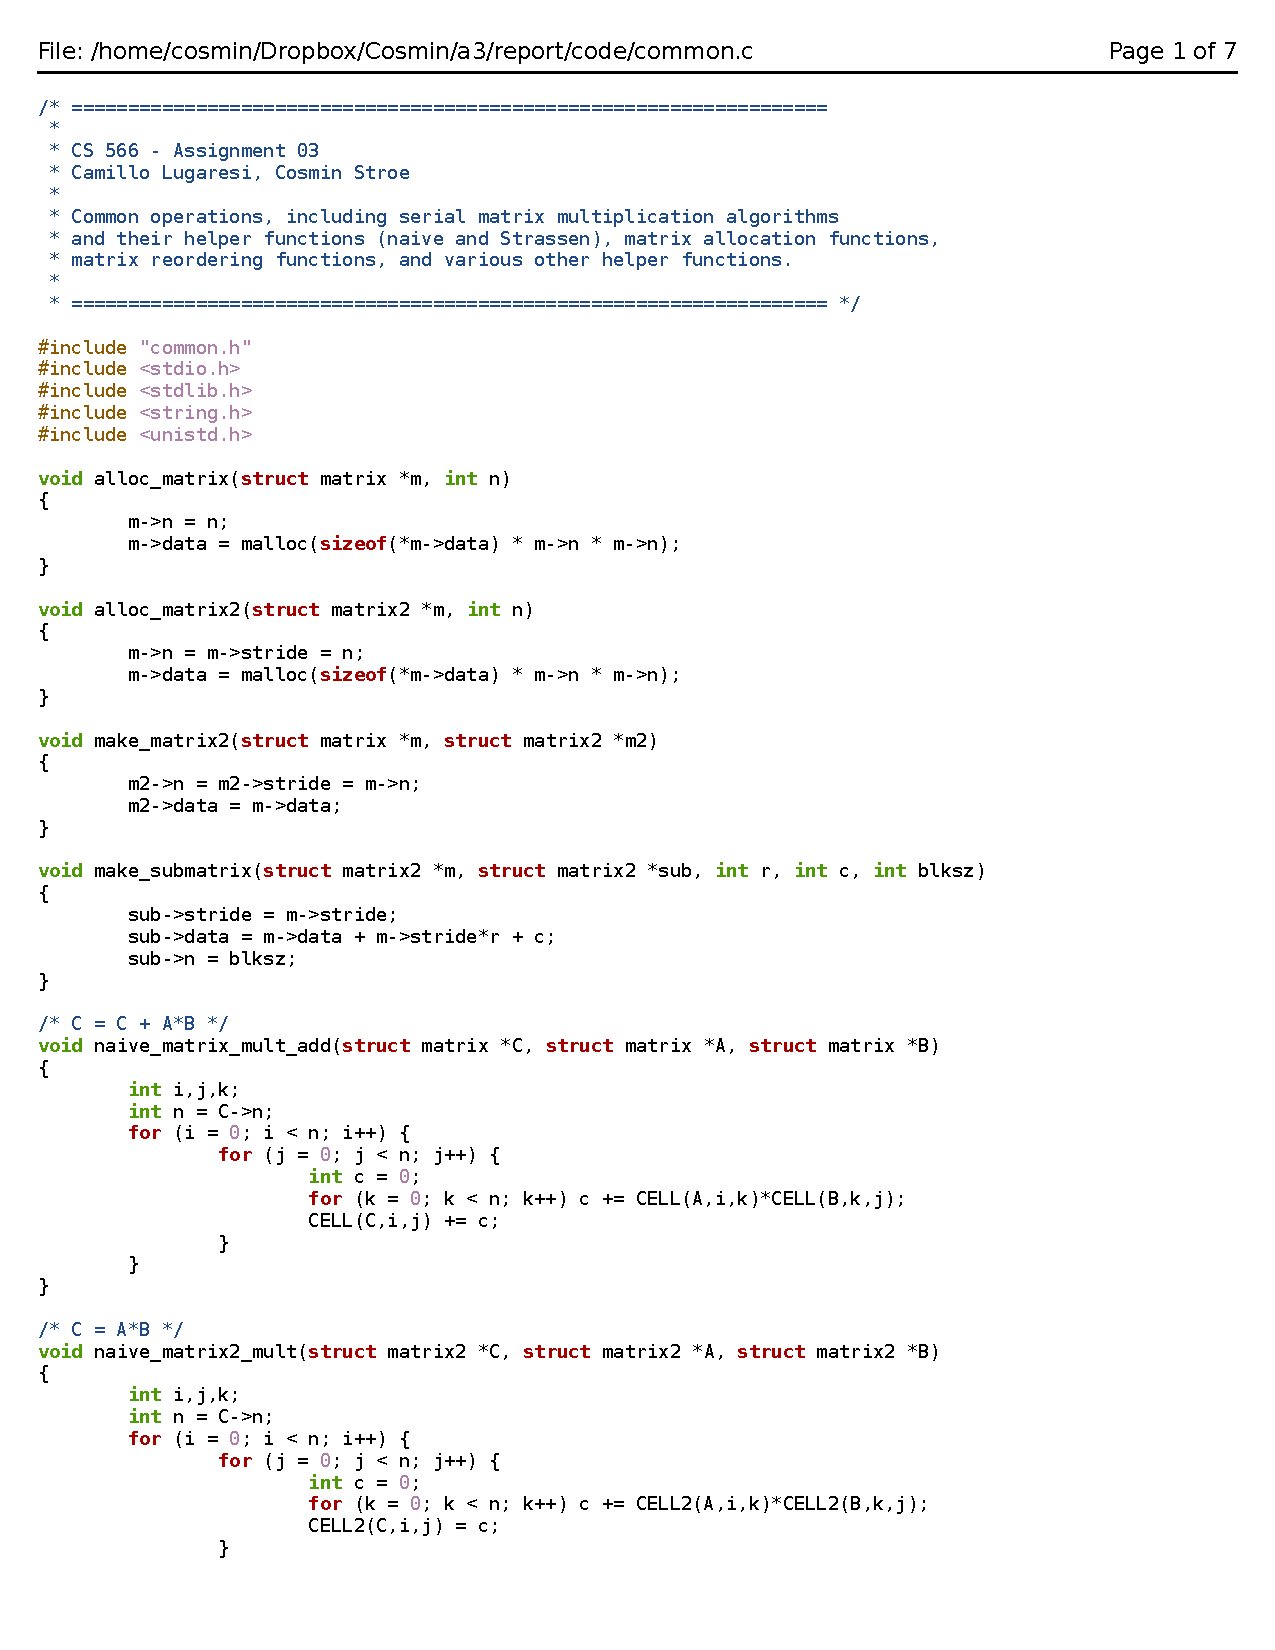
\includepdf[pages=-]{code/pdf/common-c.pdf}
% 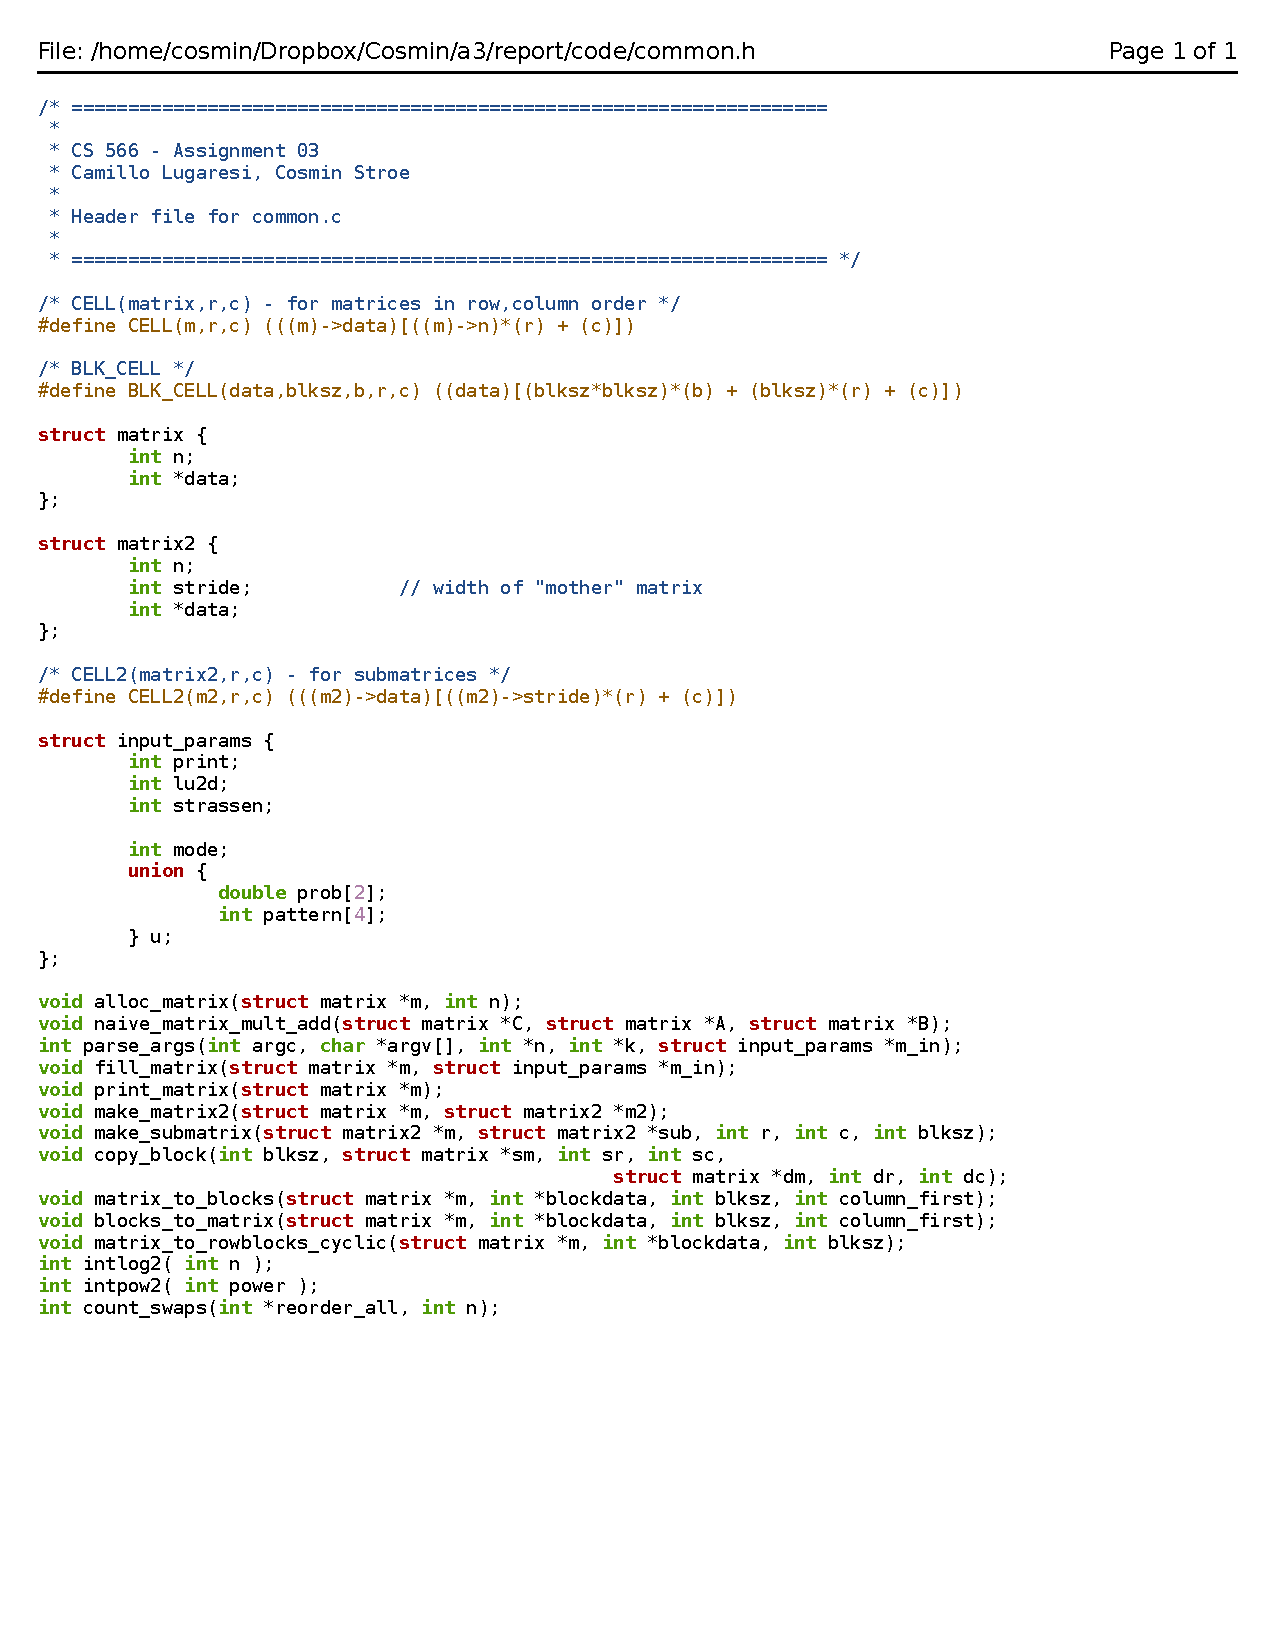
\includepdf[pages=-]{code/pdf/common-h.pdf}
% 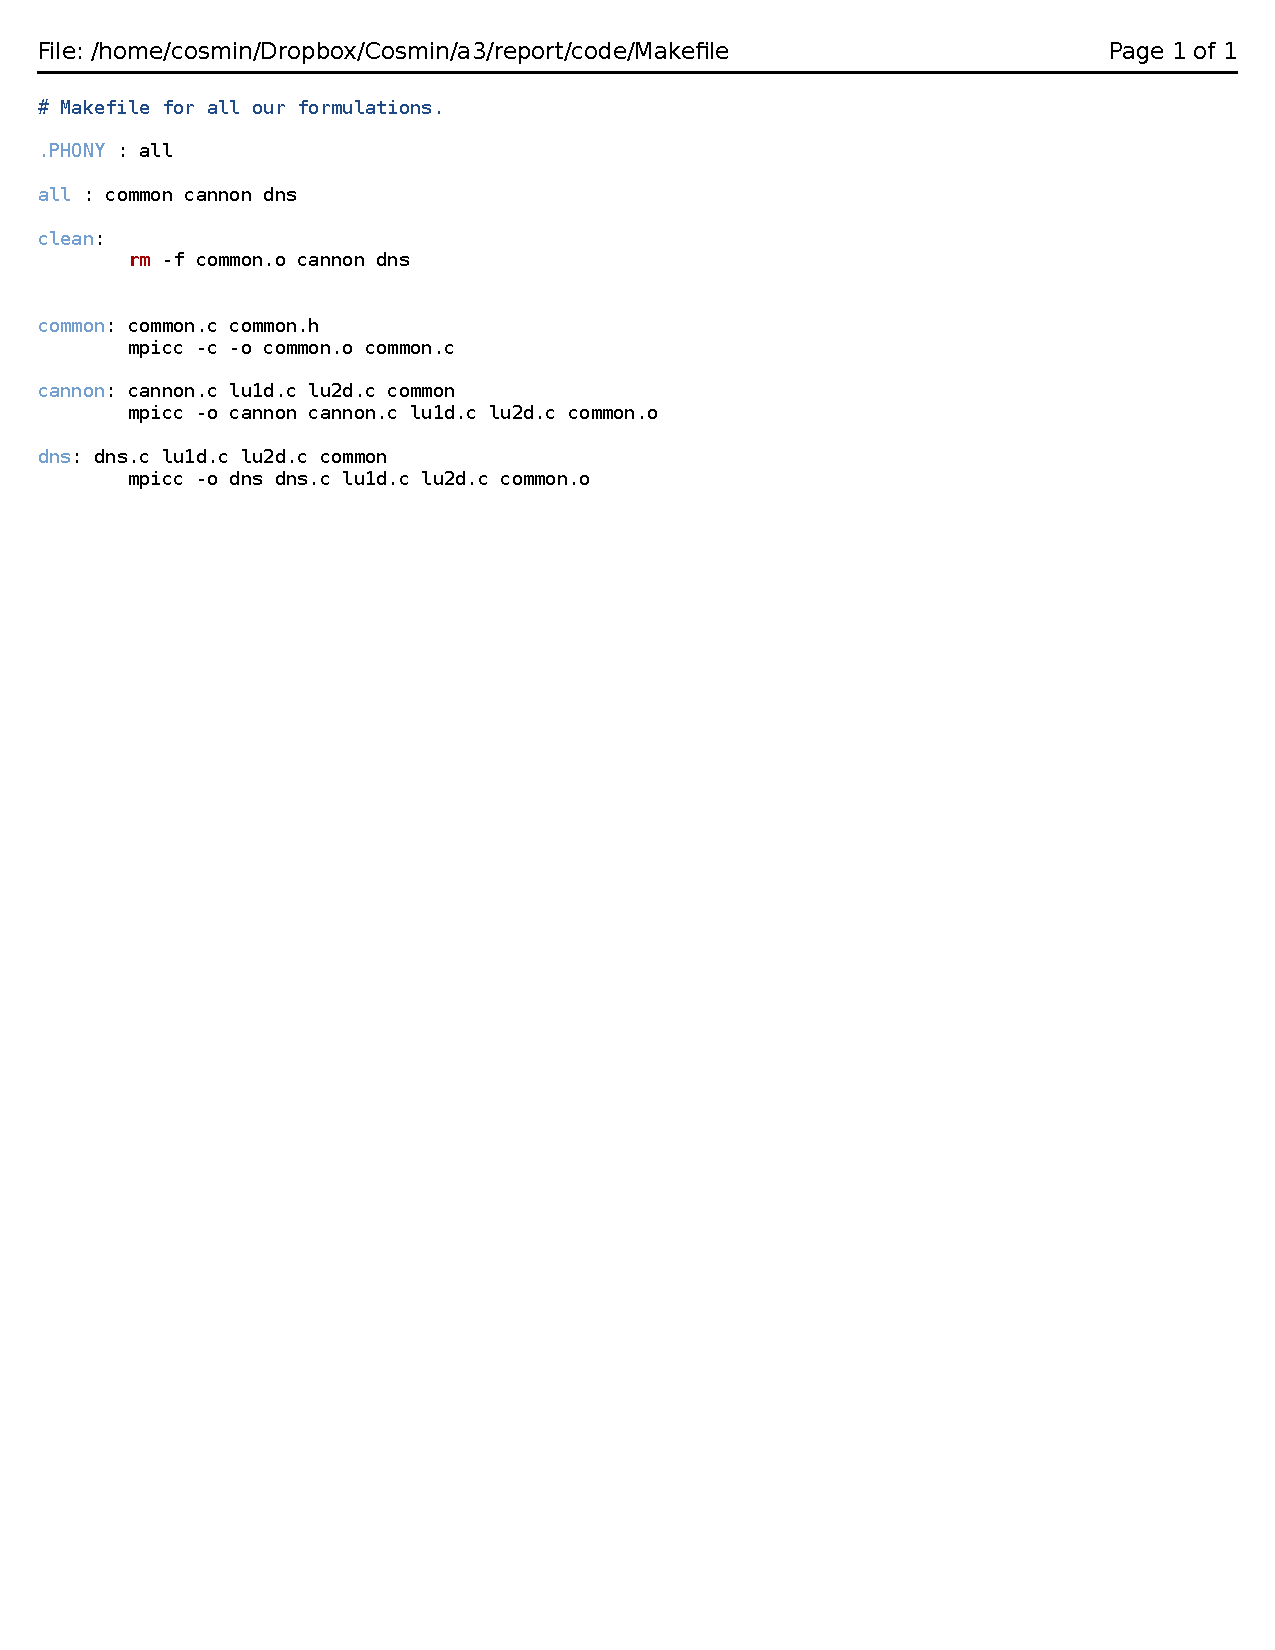
\includepdf[pages=-]{code/pdf/Makefile.pdf}

\end{document}
